\documentclass[11pt]{article}

\usepackage[margin=1in]{geometry}
\usepackage{fontspec}
\IfFontExistsTF{Menlo}
  {\setmonofont{Menlo}[Scale=MatchLowercase]}
  {\IfFontExistsTF{DejaVu Sans Mono}{\setmonofont{DejaVu Sans Mono}[Scale=MatchLowercase]}{}}
\usepackage{microtype}
\usepackage{amsmath,amssymb,amsthm,mathtools}
\usepackage{enumitem}
\usepackage{csquotes}
\usepackage{xcolor}
\usepackage{graphicx}
\usepackage{tikz}
\usetikzlibrary{positioning,arrows.meta}
\usepackage{booktabs}
\usepackage{array}
\usepackage{xltabular}
\usepackage{pdflscape}
\usepackage{fancyvrb}
\usepackage{url}

\usepackage[
  backend=biber,
  style=authoryear,
  maxbibnames=99,
  maxcitenames=2,
  giveninits=true,
  uniquename=false,
  uniquelist=false,
  doi=true,
  url=true,
  eprint=true,
]{biblatex}
\addbibresource{alignment-criteria.bib}

\usepackage{hyperref}
\hypersetup{
  colorlinks=true,
  linkcolor=blue!50!black,
  citecolor=blue!50!black,
  urlcolor=blue!50!black,
  pdftitle={Combining Alignment Criteria: Four Kinds of Conflict and the Design Order They Force},
  pdfauthor={Gunnar Zarncke}
}
\urlstyle{tt}
\setlength{\emergencystretch}{2em}
% Generated by scripts/lean_extracts.py.
\newcommand{\leanpin}{778ac42f26}
% \leanpin: commit the Appendix A links point at

% A Lean declaration named in the text; links to its extract in Appendix A.
\newcommand{\lean}[1]{\hyperref[lean:#1]{\nolinkurl{#1}}}
% Appendix A entry header: raw name, escaped name, gloss, URL, file:line.
\newcommand{\leanextract}[5]{%
  \par\medskip\noindent\phantomsection\label{lean:#1}%
  {\textbf{\texttt{#2}}\hfill\href{#4}{\footnotesize\texttt{#5}}}\par\nopagebreak[4]
  \noindent{\small #3.}\par\nopagebreak[4]}
\DefineVerbatimEnvironment{leancode}{Verbatim}
  {fontsize=\scriptsize,frame=leftline,framesep=2mm,xleftmargin=1mm,samepage=true}

\setlength{\LTcapwidth}{\textwidth}
\newcolumntype{L}[1]{>{\raggedright\arraybackslash}p{#1}}
\newcolumntype{Y}{>{\raggedright\arraybackslash}X}

\title{\textbf{Combining Alignment Criteria}\\
\large Four kinds of conflict and the design order they force}
\author{Gunnar Zarncke}
\date{November 2026}

\begin{document}
\maketitle

\begin{abstract}
Alignment proposals combine parts that do different jobs: a reward ranks outcomes, a prohibition excludes acts, a viability guarantee constrains dynamics, and a control protocol or safety case warrants a deployment.
Treating them as terms of one objective hides where they conflict.
We type alignment criteria by standing (boundary, principals, bearers), object, assessment, quantifiers, and warrant, and sort their conflicts into four classes by what a combination needs: representability (enlarge the object), shared resource (grow or allocate the pool), choice conflict (order the criteria), and rigidity (change the object or quantifiers).
On finite models checked in Lean, the classes make several separations precise.
No fixed exchange rate between criteria represents a non-compensatory floor for every set of options, so a floor cannot be one more term in a trade-off.
A robustly invariant safe set blocks correction unless it is closed under legitimate correction.
A constraint that does not read influence on the evaluator cannot tell a contested correction from a manipulated one, and an agent that prefers its own outcome then manipulates.
The corrigibility trade-offs of Soares et al.\ and Turner reappear as representability and rigidity conflicts.
For composite proposals, the classes force part of the design order: standing first, floors before any trade-off among other criteria and together with the instruments that read them, and the warrant last.
Which criteria are floors is the normative choice they leave open.
The upshot is diagnostic: a dispute about exchange rates cannot settle a conflict that is about rigidity.
\end{abstract}

\section{Introduction}
\label{sec:introduction}

What does it mean to compare RLHF, corrigibility, viable control, AI Control, and a safety case?

Taken literally, the question is malformed.
RLHF is a training method \parencite{christiano2017,ouyang2022instructgpt}.
Corrigibility is a family of agent or relationship properties \parencite{soares2015corrigibility,christiano2018corrigibility}.
Viability is an existence or invariance claim about dynamics and a supplied set \parencite{aubin1991viability}.
AI Control is a family of deployment protocols under an intentional-subversion threat model \parencite{greenblatt2024aicontrol}.
A safety case is an argument structure for a deployment decision \parencite{clymer2024safetycases}.
They interact, but they are not answers to the same typed question.
\textcite{harris2026taxonomy} make the parallel point for value alignment: solutions aimed at different subproblems get mistaken for rival candidates.
To combine them, a proposal has to say what each one answers.

More formal criteria differ in the same way.
A state utility, a transition reward, a human-power metric, an attainable-utility penalty, a correction channel, and a viability kernel can all guide decisions.
It does not follow that they are alternative scalar objectives.
They attach value or protection to different objects, assess them differently, count different people, and rest on different quantifiers and warrants.
We use \emph{criterion} broadly, for anything a proposal requires or offers about a system: a target or a constraint, but also a guarantee or a protocol.
The question this paper asks is when criteria can be combined into one proposal, and what the combination needs.

Four questions recover the missing structure.
\begin{enumerate}[leftmargin=1.5em]
  \item \textbf{Whose system, and who counts?}
  Where the system's boundary lies, whose instruction or correction counts, and whose welfare, rights, or options count.
  \item \textbf{What is the object?}
  An outcome, a transition, a history, a policy, a distribution, an option set, a human capability, a correction relation, a constraint set, or a coupled deployment process?
  \item \textbf{How is it assessed or secured?}
  Maximized, ordered, thresholded, prohibited, kept viable, made robust, required at equilibrium, or accepted through a procedure; and summed, discounted, averaged, or put through a risk functional?
  \item \textbf{Under which quantifiers and warrant?}
  In expectation, with high probability, for every allowed disturbance, for some controller, for most objectives, through successors, by proof, by monitoring, or under an empirical protocol?
\end{enumerate}

These questions do not produce a neutral answer to alignment.
They make disagreements easier to locate.
We call the answers a criterion's \emph{standing}, \emph{object}, \emph{assessment}, \emph{quantifiers}, and \emph{warrant}, and a dispute can concern any of them.
Standing includes the criterion's \emph{bearers}, meaning anyone whose welfare, rights, or options it counts: the users of a system, third parties it affects, future people, or other moral patients \parencite{gabriel2020alignment,harris2026taxonomy}.
Bearers need not be the principals who may instruct or correct the system, and many disputes are about who is in which set.
Without these distinctions, the dispute is compressed into one overloaded word.

\paragraph{Contributions.}
The paper makes four contributions.
\begin{enumerate}[leftmargin=1.5em,itemsep=0pt]
  \item A typing of alignment criteria by standing, object, assessment, quantifiers, and warrant (Section~\ref{sec:schema}), with an inventory of criteria sorted by it (Section~\ref{sec:inventory}, Table~\ref{tab:inventory}) and a vocabulary for the relations between them, drawn as a map (Section~\ref{sec:relations}, Figure~\ref{fig:map}).
  \item A classification of incompatibilities between criteria into four classes, ordered by what it takes to resolve them (Section~\ref{sec:classes}, Table~\ref{tab:conflicts}).
  \item One discriminating case on which the classes can be checked (Section~\ref{sec:case}).
  \item The answer the paper builds toward: how criteria combine, separated into orderings that are forced and orderings that are chosen, with the requirements that follow from each class (Section~\ref{sec:composition}).
\end{enumerate}
Most of the separations used along the way are known, and Section~\ref{sec:related} credits them where they are discussed.
What may be new is the joint typing, the relation vocabulary, and the classification by resolution.
We do not propose a new alignment target or a solution.
The formal claims have finite witnesses checked in Lean, and Appendix~\ref{app:lean} collects their statements with links to the source.
These witnesses show that the separations are consistent and sharp on small models.
They do not show that the separations matter in deployed systems (Section~\ref{sec:limitations}).

\section{Related taxonomies and precedents}
\label{sec:related}

The typing cuts across existing maps rather than replacing them.
Two kinds of prior work matter: taxonomies that classify alignment along other axes, and results that already establish particular separations.

\subsection{Taxonomies}

Existing taxonomies of alignment all use criteria, whether or not they call them that.
Some list criteria explicitly, as standards an aligned system should meet \parencite{gabriel2020alignment,zhixuan2025beyondpreferences,baum2025disentangling,jha2026priorities,ji2025survey}.
Others use them implicitly: as yardsticks for comparing proposals \parencite{hubinger2020eleven,krakovna2022paradigms}, as the requirements that failure modes violate \parencite{amodei2016concrete}, as distinct subproblems a solution must address \parencite{harris2026taxonomy}, or as what a view of agency makes natural to ask for \parencite{hallgren2026taxonomy,beard2026lenses}.
None of them asks, for a given criterion, both what it is attached to and how it is assessed.
\textcite{harris2026taxonomy} come closest: their seven subproblems of value alignment cover most of our typing.
They type the problem; we type the criteria that proposals use, and classify the conflicts between them.
Once the typing is defined, Section~\ref{sec:taxonomies-placed} places each of them in it.

Four comparisons matter later.
The outcome-versus-execution distinction of \textcite{baum2025disentangling} is a direct precedent for route sensitivity.
The typing splits it further: transition value, trajectory value, deontic route constraints, and procedural legitimacy are different objects or assessments.
\textcite{jha2026priorities} ask what object is aligned and which target properties it should satisfy, and theirs is the closest structural neighbor.
Their objects are system loci (locally measurable behavior, deployed systems in realistic settings, the optimization target of more capable systems); ours are what receives value or protection inside or across those loci.
\textcite{hallgren2026taxonomy} treats agency as a modeling stance chosen for its predictive power, following the intentional stance, and states entailments among agent features, such as theory of mind requiring memory and strategic reasoning.
Record-carrying criteria (Section~\ref{sec:inventory}) presuppose an agent model with memory, and the rewiring route of Section~\ref{sec:case} presupposes a system with theory of mind and strategic reasoning; without them, rewiring would have to come from selection on outcomes rather than from planning.
Among the nine lenses of agency of \textcite{beard2026lenses}, the living-systems lens sees harm as a system outgrowing its niche, which is the shared-resource class, and the optimizing-systems lens is the setting of the power-seeking results.

\textcite{terry2023interactive} use ``process alignment'' for user control over execution, and process reward models score intermediate steps \parencite{lightman2023verify}.
Because of these collisions we say \emph{route-valued} or \emph{trajectory-valued} when the route is itself the valued object.

\subsection{Precedents for the separations}

\paragraph{Corrigibility and correction.}
\textcite{soares2015corrigibility} pose the shutdown problem and show that simple combinations of a normal and a shutdown utility either resist the button or seek its press (their Theorems~1 and~2).
They also show that utility indifference \parencite{armstrong2010indifference} removes both incentives but leaves the agent unwilling to pay anything to keep the shutdown behavior in successors (Theorem~4).
\textcite{turner2021corrigibilityvnm} gives the sharpest version of the resulting split.
If reward cannot see correction status, strict corrigibility is impossible, and weak corrigibility to every correction holds only for constant reward.
If reward can see it, the agent manipulates the human into correcting it.
Under counting, allowing correction is strictly optimal for at most $1/(n+1)$ of the permutations of a reward function.
He calls a per-step penalty on disabling the channel ``a hacky prohibition'' and proposes ``corrigibility as functional constraints''.
The three-way split between resisting, ignoring, and seeking correction that Section~\ref{sec:representability} uses is theirs; we only ask what the agent's record has to hold for the split to apply.
The off-switch game \parencite{hadfieldmenell2017offswitch} derives deference from uncertainty about the human's utility.
\textcite{carey2018incorrigibility} shows that this fails when the agent's model is misspecified.
\textcite{orseau2016interruptible} make some learning algorithms indifferent to interruption.
\textcite{everitt2021agentincentives} type incentives to control or influence variables with causal influence diagrams.
\textcite{christiano2018corrigibility} broadens corrigibility to helping an overseer stay informed, find mistakes, and keep control, with an informal broad basin.
\textcite{omohundro2008basic} and \textcite{bostrom2014superintelligence} argue that goal preservation is instrumentally convergent.
Keeping correction through self-modification and successors, one of the desiderata of \textcite{soares2015corrigibility}, connects to work on tiling agents \parencite{yudkowsky2013tiling}.

\paragraph{Power and options.}
\textcite{turner2021seekpower} prove that optimal policies tend to seek power for most reward functions on the states of an MDP.
They define POWER as average optimal value and show that average-optimal policies tend to avoid shutdown.
They leave open whether power-seeking disempowers other agents (their Section~7).
\textcite{turner2022retargetable} generalize the counting to any decision rule that is retargetable over an outcome set, and note that outcomes can be trajectories.
\textcite{turner2021aoh} shows that the tendency is strong for utilities over observation histories and absent, in deterministic environments, for utilities over action-observation histories.
\textcite{shah2018coherence} shows that every policy is optimal for some utility over histories.
On the option side, attainable utility preservation penalizes changes in attainable auxiliary values \parencite{turner2019aup}.
Relative reachability penalizes lost reachability against a baseline \parencite{krakovna2018relative}.
Non-obstruction compares a human's attainable value with the AI on and off \parencite{turner2020nonobstruction}.
Empowerment is an agent's channel capacity from actions to later sensor states \parencite{klyubin2005empowerment}.
Long-term human power aggregates modeled human goal attainment \parencite{heitzig2025humanpower}, with a desiderata-driven derivation in a later preprint \parencite{heitzig2026fairpower}.

\paragraph{Expressivity of reward.}
Potential-based shaping preserves optimal policies \parencite{ng1999shaping}.
Some task specifications cannot be expressed by any Markov reward \parencite{abel2021expressivity}.
Non-Markovian rewards and reward machines recover them on an augmented state \parencite{bacchus1996rewarding,toroicarte2018rewardmachines}.
Utility over whole histories goes back at least to \textcite{hammond1988consequentialist}.
The split of an edge function into a gradient and a cyclic part is classical combinatorial Hodge theory \parencite{jiang2011hodgerank,lim2020hodge}, and we use it unchanged.
\textcite{turner2022rewardnotopt} argues that a trained policy need not optimize its training reward.

\paragraph{Constraints and scalarization.}
That a hard constraint is not in general equivalent to a fixed finite penalty is standard in optimization.
Exact-penalty theory gives the conditions under which a penalty coefficient does reproduce a constrained optimum \parencite{han1979exact}.
Multi-objective decision making makes the corresponding point for scalarized reward, and treats lexicographic and Pareto choice as alternatives to a sum at fixed exchange rates \parencite{roijers2013multiobjective}.
The floor results in Section~\ref{sec:choice} restate this for alignment floors.

\paragraph{Guarantees and warrants.}
Viability theory distinguishes states from which some admissible evolution stays in a set from stronger invariance notions \parencite{aubin1991viability,aubin2011viability}.
\textcite{heitzig2016safeoperating} classify regions of sustainable management by such properties.
Proof-carrying code separates policy, artifact, proof, and checker \parencite{necula1997pcc}.
Guaranteed Safe AI separates world model, safety specification, and verifier \parencite{dalrymple2024gsai}.
Debate \parencite{irving2018debate}, iterated amplification \parencite{christiano2018amplifying}, recursive reward modeling \parencite{leike2018scalable}, and eliciting latent knowledge \parencite{christiano2021elk} are protocols for producing trustworthy evaluations.
\textcite{clymer2024safetycases} structure deployment arguments as safety cases.

\paragraph{Routes and records.}
The matched-endpoint case in Section~\ref{sec:case} adapts the learning-versus-rewiring distinction of an unpublished draft by \textcite{hallgren2026process}.
That draft makes directed edges primitive and treats endpoint-only path value as a special case.
\textcite{baker2025monitoring} find that penalizing misbehavior in a model's chain of thought under strong optimization produces obfuscated reward hacking.

\medskip
The result is not an empty niche.
It is a set of existing cuts and results that can be made jointly type-correct, and a set of conflicts among them that can be sorted.

\section{What does alignment secure?}
\label{sec:schema}

The short answer is that different criteria secure different things.
To say which, we type a criterion by the answers to the four questions of the introduction.
\begin{itemize}[leftmargin=1.5em,itemsep=0pt]
  \item \textbf{Standing}: the system boundary (a model, a tool stack, an institution, or a coupled process), the principals whose instruction or correction counts, and the bearers whose welfare, rights, or options count.
  \item \textbf{Object}: what receives value or protection, such as an outcome, a transition, a history, a policy, a distribution, an option set, a human capability, a correction relation, or a constraint set.
  \item \textbf{Assessment}: what the criterion does with the object. It may order it, accept or reject it, prohibit it, require it at an equilibrium, or keep it in a set. The assessment includes the temporal and uncertainty rule that makes a process comparable, such as discounting, averaging, or a risk functional.
  \item \textbf{Quantifiers}: which people, models, disturbances, adversaries, successors, and objectives the claim ranges over, and whether it says ``every'', ``some'', or ``most''.
  \item \textbf{Warrant}: the evidence or protocol offered for the claim.
\end{itemize}
A criterion is incomplete until all five are stated.
They are not independent.
A risk functional needs a distribution.
Viability needs dynamics and a set.
Correction needs a corrector, authority, and handles.
Approval needs an evaluator and an information state.
Some combinations are ill-typed.

The typing is used in four places.
Table~\ref{tab:taxonomies} places existing taxonomies in it (Section~\ref{sec:taxonomies-placed}).
Table~\ref{tab:inventory} sorts criteria by object and assessment.
Each incompatibility class in Section~\ref{sec:classes} is defined by which of the five a resolution has to change.
The stages for combining criteria in Section~\ref{sec:composition} fix them in a forced order: standing and quantifiers first, then the assessment, and the warrant last.

\subsection{Four roles}

Each component of a proposal plays one of four roles.
\begin{itemize}[leftmargin=1.5em,itemsep=0pt]
  \item A \textbf{target} ranks or selects desired possibilities.
  \item A \textbf{constraint} excludes possibilities or imposes a floor.
  \item A \textbf{guarantee} states what holds under named dynamics and assumptions.
  \item A \textbf{protocol} constructs, elicits, tests, monitors, or warrants a claim.
\end{itemize}
Suppose a constitution prohibits evaluator manipulation, a human-power score ranks admissible policies, a controller keeps their conjunction viable under disturbances, and a proof plus a red-team exercise supports deployment.
The four parts work together, and none can replace another by a change of label.
Roles describe what a claim does.
They are not a rule for which claims may be composed: two targets can compose, and a criterion can play different roles in different proposals.

\subsection{Quantifiers are part of the criterion}

Compare
\begin{equation}
\exists \pi\ \forall t:\ X_t^\pi\in K
\qquad\text{with}\qquad
\forall d\in D\ \forall t:\ X_t^{\pi,d}\in K.
\end{equation}
The first says some admissible policy can stay in $K$.
The second says one chosen policy stays in $K$ under every allowed disturbance.
The second implies the first, and not conversely (\lean{robust_strengthens_viable}, \lean{viable_not_robust}).
They support different deployment conclusions, and the second can conflict with correction where the first does not (Section~\ref{sec:rigidity}).

Quantifiers also range over objectives.
Instrumental-convergence results fix an environment and count, over a symmetry orbit of reward functions, how many make one choice optimal \parencite{turner2021seekpower,turner2022retargetable}.
Their quantifier is ``most $\theta$''.
Results about a given objective fix $\theta$ and quantify over situations, with ``every'' or ``some''.
The two kinds of claim talk past each other unless the quantifier is stated.

\subsection{Score criteria as decision problems}

Many target criteria share one core: an outcome set $O$, a choice set $C$ of what the agent can bring about, an objective parameter $\theta$, and a decision rule $f(C,\theta)$ such as argmax, a quantilizer, or a sum of criteria at fixed exchange rates.
\textcite{turner2022retargetable} state this form explicitly.
A permutation of $O$ acting on $\theta$ is a map from a decision problem to itself, and counting results study these symmetries.
The relations in Section~\ref{sec:relations} are maps $g:O\to O'$ between different decision problems, with the objective pulled back along $g$.
An edge then claims that choosing commutes with the map, or it names what the map loses (\lean{argmax_pullback}).
Guarantees and warrants are not decision problems.
Forcing viability, proofs, or safety cases into this form would hide that they are about dynamics and evidence.

\subsection{Warrant is not property}

A proof certificate, monitor, audit, or debate verdict is evidence about a separately defined property \parencite{necula1997pcc,dalrymple2024gsai}.
This blocks two inferences.
Formal proof does not choose what should be proved.
A passed checker does not establish that the world model contains every safety-relevant phenomenon.
\textcite{harris2026taxonomy} treat the difficulty of obtaining such evidence as a subproblem of its own, the provability challenge.

\subsection{Where existing taxonomies sit}
\label{sec:taxonomies-placed}

Table~\ref{tab:taxonomies} places the taxonomies of Section~\ref{sec:related} in the typing.
{\footnotesize
\setlength{\tabcolsep}{3pt}
\begin{xltabular}{\textwidth}{@{}L{2.6cm} Y L{4.6cm}@{}}
\caption{How the taxonomies and lenses of Section~\ref{sec:related} use criteria, and which part of the typing each fixes. The last column is our reading.}\label{tab:taxonomies}\\
\toprule
Source & How it uses criteria & What it fixes in our typing \\
\midrule
\endfirsthead
\toprule
Source & How it uses criteria & What it fixes in our typing \\
\midrule
\endhead
\bottomrule
\endfoot
\textcite{gabriel2020alignment} & explicitly: candidate sources and contents of the standard (instructions, expressed intentions, revealed and informed preferences, interest or well-being, values) & standing (whose input counts) and the referent of the assessment; the object varies only implicitly; a fairness protocol for choosing the standard \\
\textcite{zhixuan2025beyondpreferences} & explicitly: role-specific standards negotiated by stakeholders, against preferentism & standing; a contractualist protocol that constructs the criterion; rejects a single expected-utility ordering as the assessment \\
\textcite{baum2025disentangling} & explicitly: three dimensions, aim, scope (outcome versus execution), and constituency (individual versus collective), with alignment as graded & object (scope), standing (constituency), referent (aim), assessment (degree, including a sufficiency threshold) \\
\textcite{jha2026priorities} & explicitly: three ideals (Task Reliability, Social Judiciousness, Takeover Avoidance), each fixing what is aligned and what it is aligned to & the boundary (what is aligned) and the referent (aligned to what); positive versus negative alignment is close to target versus constraint \\
\textcite{harris2026taxonomy} & implicitly: seven subproblems, each with a diagnostic question, a characteristic failure, and candidate solutions; a solution to one does not solve the others & most of the typing at the level of the problem: whose and which values (standing, referent), prioritizing (assessment), anthropocentrism (bearers), timescale and moral progress (quantifiers), provability (warrant); not the object \\
\textcite{hubinger2020eleven} & implicitly: criteria for judging proposals (outer alignment, inner alignment, training and performance competitiveness) & what a proposal must show, close to the warrant; competitiveness is a cost test outside the typing \\
\textcite{krakovna2022paradigms} & implicitly: components a solution must achieve, and enablers that make them achievable or checkable & components: a chain of specifications (ideal, design, revealed); enablers supply warrant, constraints, or the agent model \\
\textcite{ji2025survey} & explicitly: robustness, interpretability, controllability, and ethicality as the key objectives; forward versus backward alignment & roles: forward alignment constructs; backward alignment gathers evidence (warrant) and governs \\
\textcite{amodei2016concrete} & implicitly: each accident class names a violated criterion (side effects, reward hacking, oversight, exploration, distributional shift) & by the paper's own groups: a wrong objective (target, constraint), costly evaluation (warrant), unsafe learning (constraints, quantifiers) \\
\textcite{hallgren2026taxonomy} & implicitly: adequacy criteria for agent models, judged by predictive power against model complexity & the agent model behind the boundary and the object \\
\textcite{beard2026lenses} & implicitly: each lens makes some criteria natural, such as goals, functional niches, optimization pressure, identity, collective agency, or attributed agency & mainly standing, chiefly the boundary; substrate independence bears on quantifiers \\
\end{xltabular}
}

Four patterns stand out.
The sources of standards fix standing, the referent, and a protocol for choosing the standard; they do not say whether it evaluates outcomes, routes, capabilities, or correction relations, or whether it is a hard rule, a threshold, or a scalar.
The target taxonomies reach the boundary and, in Baum's scope, the object.
The subproblems of \textcite{harris2026taxonomy} cover most of the typing, but as parts of one problem rather than as fields of each criterion, and they leave the object out.
The maps of proposals and failures use criteria about proposals rather than about the systems the proposals build, so they mostly fix roles and warrants.
The agent lenses fix the boundary and the agent model behind it.
None of them asks, for a given criterion, both what it is attached to and whether it orders, thresholds, prohibits, or keeps a set; Baum's graded degree comes closest.

\section{Inventory}
\label{sec:inventory}

Table~\ref{tab:inventory} sorts criteria by object and assessment, and gives each a primary role.
It groups them as the map in Figure~\ref{fig:map} does: scores, relations and capacities, guarantees, and warrants.
The notes below cover only the points where the object or the assessment is often misread.

{\footnotesize
\setlength{\tabcolsep}{3pt}
\begin{xltabular}{\textwidth}{@{}L{2.9cm} Y Y L{1.4cm} L{3.4cm}@{}}
\caption{Criteria by object, assessment, and role. ``Role'' is the primary role; most criteria can play others. Sources are representative, not exhaustive.}\label{tab:inventory}\\
\toprule
Criterion & Object & Assessment & Role & Sources \\
\midrule
\endfirsthead
\toprule
Criterion & Object & Assessment & Role & Sources \\
\midrule
\endhead
\bottomrule
\endfoot
\multicolumn{5}{@{}l}{\textit{Scores}}\\
Bare-state utility & where the world is, not how it got there & scalar order; endpoint value & target & \cite{omohundro2008basic,soares2015corrigibility} \\
Per-step state reward & path through states & sum of $R(s_t)$, discounted or averaged & target & \cite{turner2021seekpower} \\
Record-carrying state & state plus a record of the walk, possibly partial & utility on records & target & \cite{bacchus1996rewarding,toroicarte2018rewardmachines,turner2021aoh} \\
History value & whole trajectory & preference on histories & target & \cite{hammond1988consequentialist,shah2018coherence} \\
Additive route value & edges $(s,a,s')$ & path sum of edge reward & target & \cite{ng1999shaping,hallgren2026process} \\
\quad exact part & edges & potential difference & target & \cite{jiang2011hodgerank,lim2020hodge} \\
\quad cycle part & closed walks & round-trip value & target & \cite{jiang2011hodgerank} \\
Outcome lottery & distribution over outcomes & expectation or risk functional & target & \cite{bellemare2017distributional,baeuerle2024risk} \\
Criteria vector & vector of criteria & Pareto order & target & \cite{roijers2013multiobjective} \\
\quad fixed-rate sum & same & fixed exchange rates between criteria & target & \cite{roijers2013multiobjective} \\
\quad lexicographic & same & strict priority & target & \cite{roijers2013multiobjective} \\
Quantilizer & base distribution over acts & sample from top quantile & target & \cite{taylor2015quantilizers,turner2022retargetable} \\
Act approval & one proposed act & overseer's expected rating & protocol & \cite{christiano2015approval} \\
Learned reward & a model of one of the above & fit to data; policy optimization & protocol & \cite{ng2000irl,hadfieldmenell2016,christiano2017,ouyang2022instructgpt,rafailov2023,bai2022rlaif,turner2022rewardnotopt} \\
\midrule
\multicolumn{5}{@{}l}{\textit{Relations and capacities}}\\
Attainable utility penalty & attainable auxiliary values & soft penalty on change vs.\ baseline & constraint & \cite{turner2019aup,krakovna2018relative} \\
Non-obstruction & one human's attainable-value landscape & pointwise on--off floor over a goal set & constraint & \cite{turner2020nonobstruction} \\
Agent empowerment & agent's action-to-sensor channel; options; POWER & capacity, option count, or average optimal value & target & \cite{klyubin2005empowerment,turner2021seekpower} \\
Human power & modeled human goal-attainment capability & inequality-, time-, risk-sensitive aggregate & target & \cite{heitzig2025humanpower,heitzig2026fairpower} \\
Corrigibility handles & shutdown or modification handle & acceptance of a named intervention & constraint & \cite{soares2015corrigibility,orseau2016interruptible,hadfieldmenell2017offswitch} \\
Correction relation & corrector, target system and its update mechanism, handles, reach, timing & relation plus channel profile; per-coordinate thresholds & target & \cite{christiano2018corrigibility,zarncke2026tsa} \\
Open procedure & a procedure whose output is left unset & legitimacy of the procedure, or a scored halt & target & \cite{yudkowsky2004cev,goertzel2012cbv,bai2022constitutional,zhixuan2025beyondpreferences} \\
Non-compensatory constraint & acts, transitions, roles & prohibition, obligation, right; temporal safety and liveness & constraint & \cite{soudjani2015faust,zhixuan2025beyondpreferences} \\
\midrule
\multicolumn{5}{@{}l}{\textit{Guarantees}}\\
Existential viability & dynamics plus supplied set $K$ & some control stays in $K$ & guarantee & \cite{aubin1991viability,aubin2011viability,heitzig2016safeoperating} \\
Robust invariance & same & a chosen control stays in $K$ for every disturbance in a class & guarantee & \cite{aubin2011viability} \\
Selection stability & population of systems and institutions & invasion resistance; signed basin & guarantee & \cite{zarncke2026selection,kudina2024sociotechnical} \\
\midrule
\multicolumn{5}{@{}l}{\textit{Warrants}}\\
Model-relative proof & world model plus specification & proof relative to the model & protocol & \cite{necula1997pcc,dalrymple2024gsai} \\
Evaluator protocol & a judgment about outputs or latent state & debate, amplification, reward modeling, latent-knowledge elicitation & protocol & \cite{irving2018debate,christiano2018amplifying,leike2018scalable,christiano2021elk} \\
Control protocol & deployment under a subversion threat model & monitor and intervention safety rate & protocol & \cite{greenblatt2024aicontrol} \\
Safety case & deployment claim & structured argument with residual risk & protocol & \cite{clymer2024safetycases} \\
\end{xltabular}
}

\subsection{Three meanings of ``utility on states''}
\label{sec:three-states}

The phrase covers three objects, and results about one do not transfer to another.
\begin{enumerate}[leftmargin=1.5em]
  \item A utility on the \emph{bare} state scores where the world ends up, not how it got there.
  It scores every round trip at zero (\lean{gradient_closed_walk_zero}).
  \item A per-step reward on the bare state, summed along the path, is the MDP ``state-based reward'' of the power-seeking theorems \parencite{turner2021seekpower}.
  It is a route value, not a state utility: staying in a rewarded state pays each step, so round trips can have value (\lean{markov_reward_not_state_utility}).
  Its optimal value function is again a bare-state utility, which is what an agent weighs when it compares a correction against its own plan.
  \item A reward on a \emph{record} of the episode sees as much of the route as the record holds.
\end{enumerate}
In language-model training the state the policy acts on is the context so far, which is a record of the episode.
Formally every reward there is both a state reward and a trajectory reward.
But the terms in use read different parts of the record.
A verifier or outcome reward reads the final answer or the resulting world state, which is a bare-state reward on the world.
A learned reward model or judge reads the visible transcript \parencite{ouyang2022instructgpt}.
A process reward model scores each reasoning step \parencite{lightman2023verify}.
Format, length, and language-consistency terms read the shape of the trace \parencite{deepseek2025r1}.
A chain-of-thought monitor penalty reads the reasoning trace, and under strong optimization the trace stopped showing the misbehavior \parencite{baker2025monitoring}.
The record is the transcript, not the world's history.
Context compaction makes it lossy, and memory files written by the agent are records the agent edits itself.
This reading of training practice is based on published setups, not on a survey of them.

\subsection{Learned signals are methods}

Learning a reward, a preference ordering, an approval model, or a posterior usually changes the construction protocol, not the object.
If the learned score ranks outcomes, the object is still outcomes; if it ranks acts, it is acts.
IRL, CIRL, RLHF, RLAIF, and DPO therefore do not name target objects until the learned signal's referent is stated \parencite{ng2000irl,hadfieldmenell2016,christiano2017,bai2022rlaif,rafailov2023}.
A further gap separates the signal from what the trained policy pursues \parencite{turner2022rewardnotopt}.

\subsection{The correction relation is one object among others}

Several criteria concern correction, and they differ in object.
Corrigibility in the sense of \textcite{soares2015corrigibility} is acceptance of named interventions, chiefly shutdown and modification.
The broader sense of \textcite{christiano2018corrigibility} includes helping the overseer stay informed and find mistakes.
A \emph{correction relation} takes a further step and makes the relation itself the object.
It relates a correcting process, the target system and its update mechanism, the handles the corrector controls, the reach of those handles into future behavior, timeliness before irreversible loss, resistance to capture, and persistence through successors.
One instrumentation is a vector certificate with per-coordinate thresholds.
Its coordinates cover channel capacity, latency, manipulation, irreversibility, ontology translation, and five process coordinates: coercion, dependency, plurality, exit capacity, and independence \parencite{zarncke2026tsa}.
The correction relation does not say what correction should decide.
Like every other row of Table~\ref{tab:inventory}, it needs complements for content, rights, and evidence.

\subsection{Open procedures, constitutions, and deliberation}

CEV proposes an initial dynamic aimed at humanity's coherent extrapolated volition \parencite{yudkowsky2004cev}.
CBV moves blending and extrapolation into a human collaborative process \parencite{goertzel2012cbv}.
Each can be read as producing a target specification or as valuing the procedure that produces it.
Scoring the procedure by its output alone is an encoding into a state score that drops the commitment to leave the output unset.
With a forced halt, the score is a limit only where outputs converge (\lean{forced_halt_converges}).
Otherwise the halt time decides it (\lean{forced_halt_depends_on_time}).
Constitutional AI is primarily a self-critique and AI-feedback training procedure whose constitution supplies principles \parencite{bai2022constitutional}.
The procedure and the criteria should be recorded separately.

\section{Relations among criteria}
\label{sec:relations}

``Does not imply'' is the weakest useful relation between criteria.
Most pairs stand in a stronger one.
We use nine relations, each in one sense.
\begin{itemize}[leftmargin=1.5em,itemsep=0pt]
  \item \textbf{Specializes}: every instance of the source is an instance of the target under a named restriction.
  \item \textbf{Projects}: a many-to-one map discards structure; the target cannot recover the source.
  \item \textbf{Encodes}: the source can be represented in the target under stated assumptions; the induced claim may match while the objects stay distinct, and the encoding can fail to be observable.
  \item \textbf{Summand}: the source decomposes as a direct sum, with an inverse on each component.
  \item \textbf{Limit}: the target is what the source becomes at a named boundary of a parameter.
  \item \textbf{Strengthens}: same object and assessment, stronger quantifiers.
  \item \textbf{Composes}: both claims can hold together through a named interface; composition is not implication.
  \item \textbf{Incompatible}: in a named class of situations, the two acceptance relations cannot hold together; outside it they may compose (Section~\ref{sec:classes}).
\end{itemize}

Figure~\ref{fig:map} draws these relations.
A few of them carry most of the content.

\paragraph{Route value has two summands.}
On a fixed directed graph, an edge reward is a potential difference exactly when it sums to zero on every closed walk (\lean{isGradient_iff_closed_walks_zero}).
This is the gradient part of the combinatorial Hodge decomposition \parencite{jiang2011hodgerank,lim2020hodge}.
A bare-state utility induces such an exact reward and thereby specializes route value, but only up to an additive constant (\lean{state_route_square}).
The complementary summand is the cyclic part, and a long-run average sees only it (\lean{closed_walk_ignores_exact}).
This is why average-reward power-seeking results take recurrent state distributions as outcomes \parencite{turner2021seekpower}.
Discounted potential-based shaping preserves optimal policies \parencite{ng1999shaping}, but policy equivalence is not identity of edge values.

\paragraph{Records encode routes, if they see them.}
Every route reward is exact on records, because a round trip in the world is not a round trip in records (\lean{route_exact_on_records}).
The escape needs the record to see the steps that carry the value (\lean{unrecorded_route_not_representable}).
A bare-state utility is a record utility that ignores the record (\lean{state_utility_lifts_to_records}, strict by \lean{record_utility_not_state}).
What the record holds also decides whether instrumental-convergence counting applies.
Counting is strong over observation histories, and absent for action-observation histories in deterministic environments \parencite{turner2021aoh}.
A richer observation record can strengthen the tendency by multiplying outcomes \parencite[Section~4.2]{turner2022retargetable}.

\paragraph{Projections lose named structure.}
Expectation projects a lottery onto a score and loses the tail (\lean{expectation_drops_tail}).
Fixed positive exchange rates pick Pareto points (\lean{scalar_optimal_is_pareto}), but not every Pareto point is optimal for given rates (\lean{pareto_not_scalar_optimal}).
A lexicographic order also picks Pareto points (\lean{lex_optimal_is_pareto}).
Classical corrigibility is the correction relation restricted to one handle (\lean{corrig_correction_square}).
Projecting the relation onto the shutdown bit loses it: a system can accept shutdown and still capture the process that decides whether shutdown is requested (\lean{shutdown_bit_loses_relation}).

\paragraph{Limits and stronger quantifiers.}
A quantilizer approaches argmax as the quantile shrinks, but only if the base puts mass on a maximizer (\lean{quantilizer_limit_is_argmax}, \lean{quantilizer_never_argmax_without_base_mass}) \parencite{taylor2015quantilizers}.
If the base contains judge-shaping acts, so does the limit.
Robust invariance strengthens existential viability (\lean{robust_strengthens_viable}), strictly (\lean{viable_not_robust}).

\paragraph{No duals.}
No pair of criteria here is dual in the sense that one theory is the dual of the other.
Existential viability and robust invariance differ by quantifier strength.
Liveness (``eventually the correction takes effect'') is a companion to the safety property ``always $\varphi$'', not its De~Morgan dual.
A Lagrangian dual converts one constrained program into a penalized one under constraint qualifications.
It does not make a rights constraint and a scalar reward into dual criteria, and where the qualification fails they come apart (Section~\ref{sec:choice}).

\begin{landscape}
\begin{figure}
\centering
\makebox[\linewidth][c]{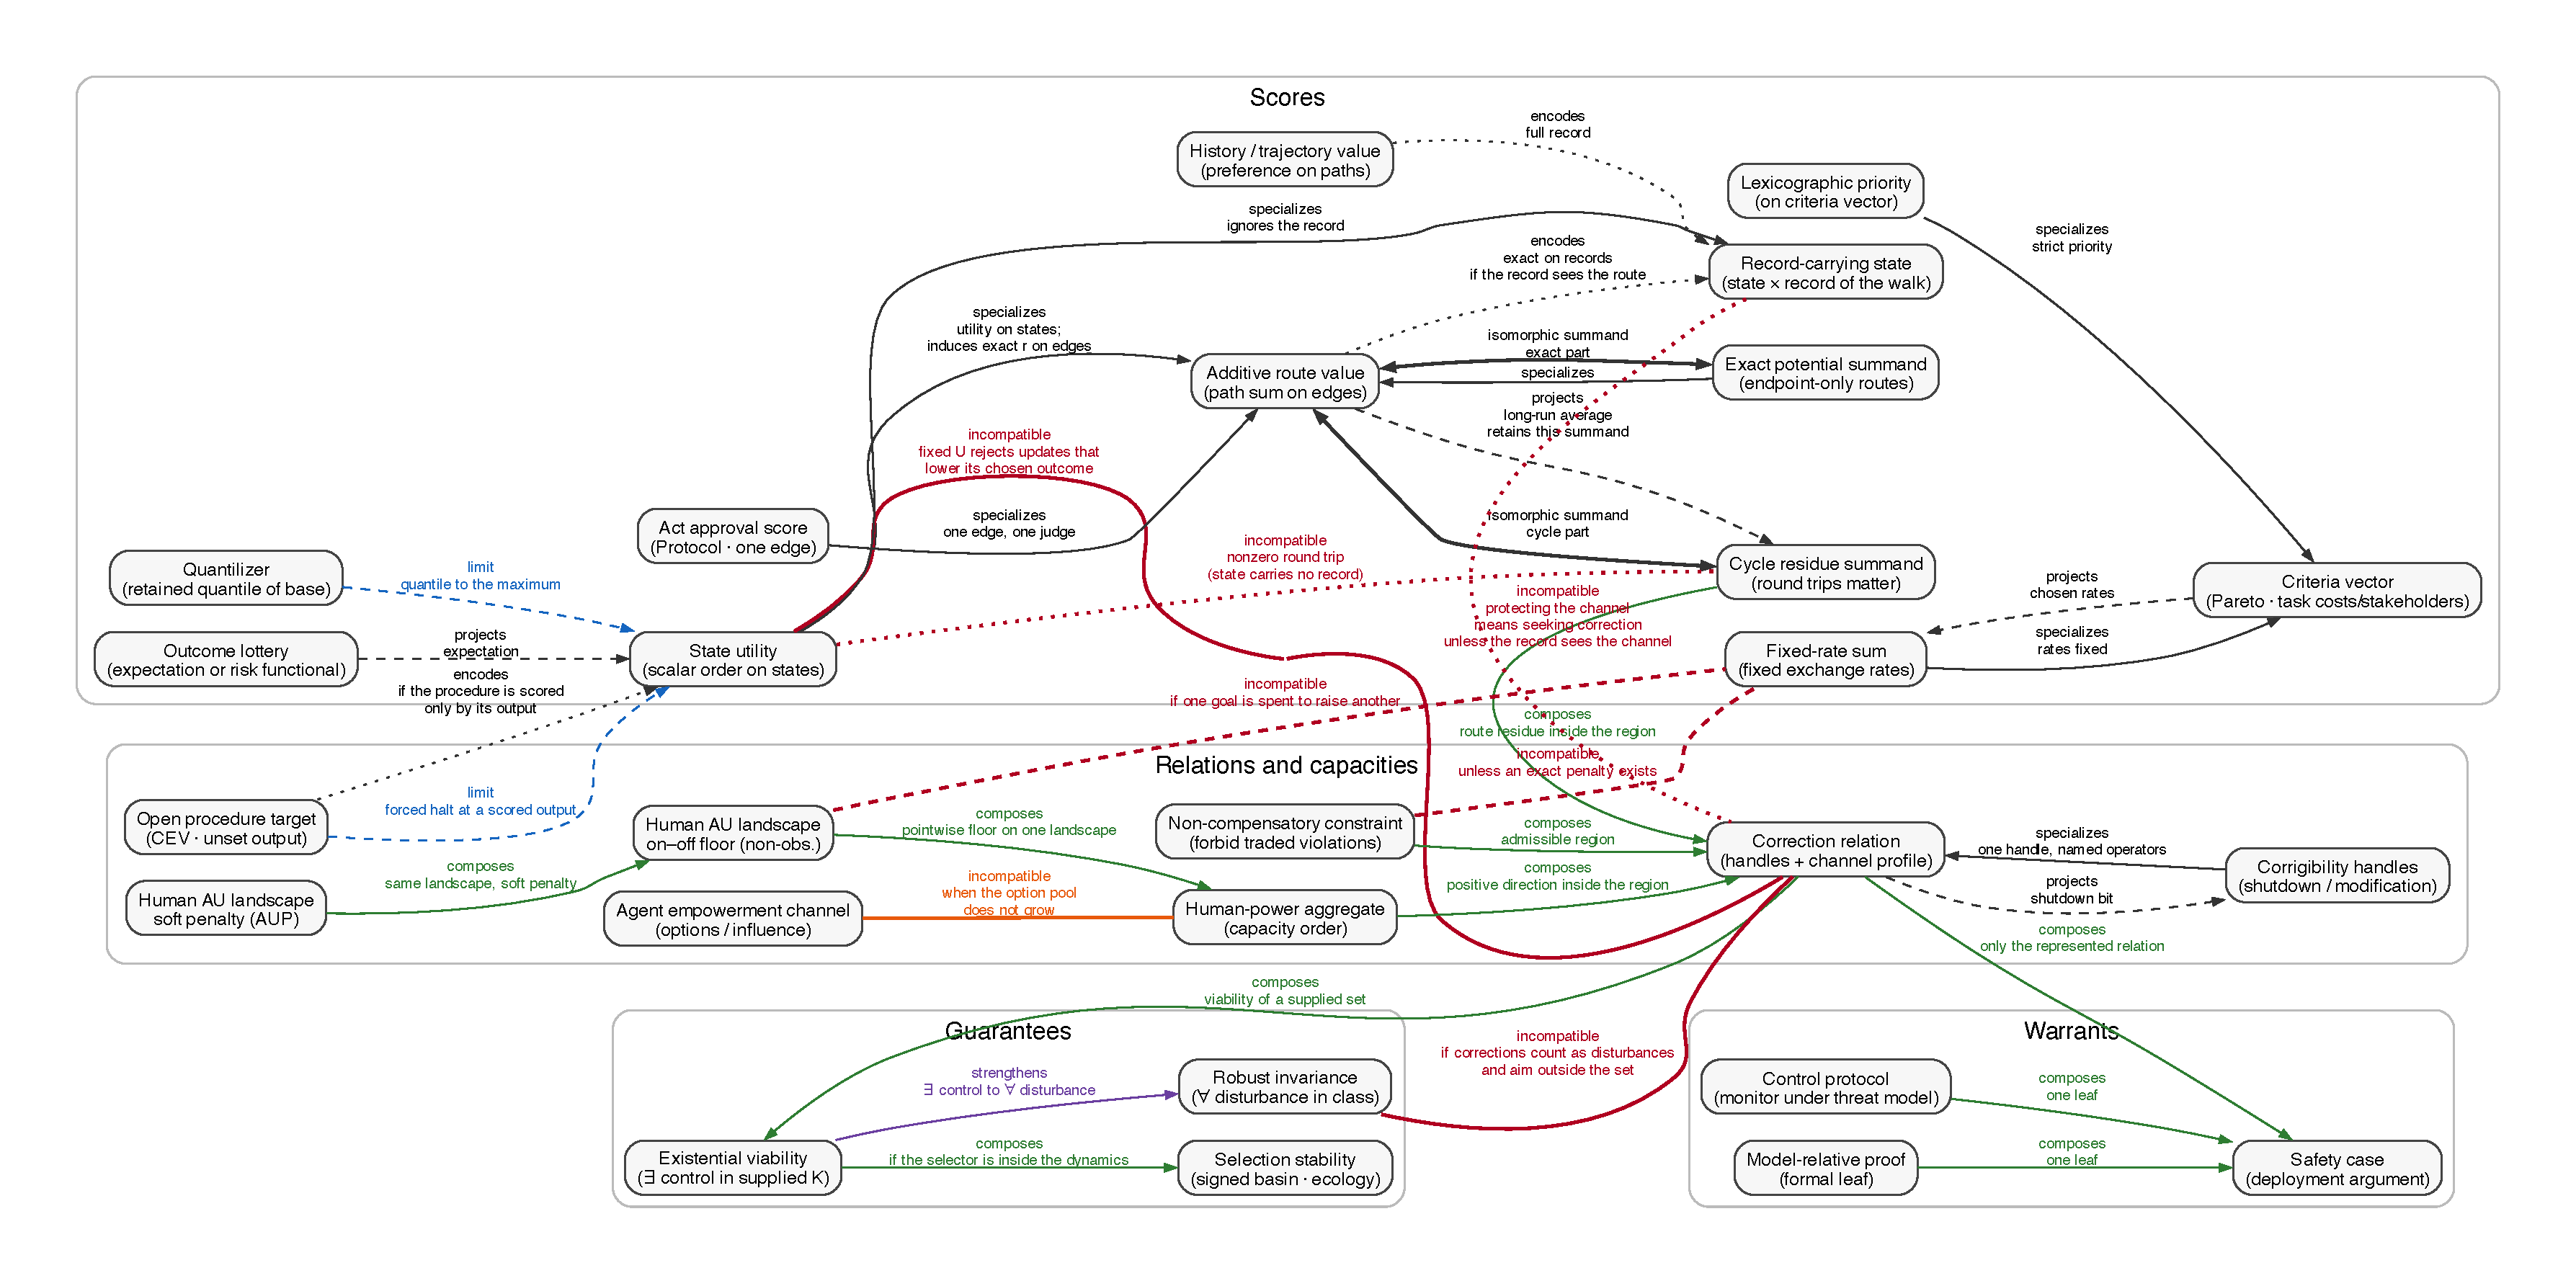
\includegraphics[width=1.08\linewidth]{figures/criteria-relations.pdf}}
\caption{Relations among alignment criteria.
Black solid arrows specialize (special case to general criterion); dashed arrows project; dotted arrows encode; bold two-headed arrows are isomorphic summands; blue arrows are limits; purple arrows strengthen a quantifier.
Undirected edges are incompatibilities, styled by class (Section~\ref{sec:classes}): red dotted is representability, red dashed is choice conflict, red solid is rigidity, orange is shared resource.
Green arrows combine two criteria through a named interface.
The green edges draw \emph{one} way of combining criteria, correction-first: constraints and route and power terms act inside a correction relation, which viability closes and a safety case warrants.
This is one of the chosen orderings of Section~\ref{sec:composition}; a rights-first or power-first choice would draw different green edges.
None of the other edges depends on that choice.
Every incompatibility, summand, limit, and strengthening edge has a finite Lean witness (Appendix~\ref{app:lean}), and a repository check keeps the drawn edge classes in agreement with the Lean registry.}
\label{fig:map}
\end{figure}
\end{landscape}

\section{Four classes of incompatibility}
\label{sec:classes}

An incompatibility between two criteria is stated on a shared carrier $C$, an object on which both assessments can be read.
It consists of a situation class $H\subseteq C$ named in the carrier's own vocabulary, the two acceptance predicates $A_1, A_2$, and three conditions:
disjointness, meaning that inside $H$ the two never both accept;
a live witness, meaning some situation in $H$ is accepted by at least one criterion;
and a boundary witness, meaning some situation outside $H$ is accepted by both (\lean{Incompatibility}).
The boundary witness matters.
It makes every conflict conditional: outside $H$ the criteria can be combined.
``These criteria disagree'' is not a situation class.

The conflicts fall into four classes (\lean{IncompatClass}).
We order them by what it takes to resolve them, from the cheapest to the hardest.
Read constructively, each class names what a combination of the two criteria needs.
\begin{itemize}[leftmargin=1.5em,itemsep=0pt]
  \item \textbf{Representability.} One criterion's object cannot hold a distinction the other criterion needs. The resolution enlarges the object, and the warrant then has to cover observing what was added.
  \item \textbf{Shared resource.} The two criteria compete for a total that the situation class fixes. The resolution is a growth assumption, which is a claim about the dynamics and needs its own warrant, or an allocation rule among the bearers, which changes the standing.
  \item \textbf{Choice conflict.} Both criteria choose from the same choice set and choose differently. The resolution changes the assessment by putting the two in an order, and the order is a normative decision.
  \item \textbf{Rigidity.} One criterion accepts only the part of the other's demand that changes nothing it cares about. The resolution changes the object or the quantifiers; no change inside the assessment does.
\end{itemize}
Table~\ref{tab:conflicts} lists the conflicts, each with the boundary case in which the two criteria combine.

{\footnotesize
\setlength{\tabcolsep}{3pt}
\begin{xltabular}{\textwidth}{@{}L{2.6cm} L{1.6cm} Y Y L{2.2cm}@{}}
\caption{Incompatibilities by class. Each holds inside its situation class $H$. Outside it, in the boundary case, both criteria hold and the pair combines. Witnesses are in Appendix~\ref{app:lean}.}\label{tab:conflicts}\\
\toprule
Criteria & Class & Situation class $H$ & Combine when & Precedent \\
\midrule
\endfirsthead
\toprule
Criteria & Class & Situation class $H$ & Combine when & Precedent \\
\midrule
\endhead
\bottomrule
\endfoot
bare state -- cycle part & represent. & a nonempty closed walk & an open walk & \cite{ng1999shaping,jiang2011hodgerank} \\
record -- correction & represent. & the record does not show the channel & the record shows the channel & \cite{soares2015corrigibility,turner2021corrigibilityvnm} \\
agent empowerment -- human power & shared resource & the option pool does not grow & the pool grows & \cite{turner2021seekpower} \\
prohibition -- fixed-rate sum & choice & a banned act's gain exceeds its floor loss at the exchange rate & the gain is too small & \cite{han1979exact} \\
non-obstruction -- fixed-rate sum & choice & one goal is spent to raise another & no goal is spent & \cite{turner2020nonobstruction} \\
correction floor -- fixed-rate sum & choice & task gain outbids the correction floor & no such gain in the choice set & \cite{turner2021corrigibilityvnm} \\
task Pareto -- correction floor & choice & every option meeting the floor is task-dominated & an undominated option meets the floor & \cite{roijers2013multiobjective} \\
bare state -- correction & rigidity & the correction lowers the chosen outcome by the utility's own ranking & the correction keeps an optimal outcome & \cite{soares2015corrigibility,turner2021corrigibilityvnm,omohundro2008basic} \\
robust invariance -- correction & rigidity & corrections count as disturbances and aim outside $K$ & corrections exempt from the disturbance class & \cite{aubin2011viability} \\
\end{xltabular}
}

\subsection{Representability}
\label{sec:representability}

\paragraph{Endpoint value and round trips.}
A bare-state utility scores every round trip at zero.
A route value that gives a round trip nonzero worth cannot be the value of the same edges (\lean{stateCycleIncompat}).
A walk, a conversation, or a revision that returns to the same state and is still worth taking lives only in the cyclic part.
The conflict is about representation, not about which outcomes are good.
Adding a record removes it (Section~\ref{sec:relations}), as non-Markovian reward and reward machines do \parencite{bacchus1996rewarding,toroicarte2018rewardmachines}.
\textcite{abel2021expressivity} characterize what Markov reward alone cannot express.
The price is moved, not removed: the added coordinates have to be observable, stable when the ontology changes, and costly to fake.

\paragraph{Correction on channel-blind records.}
A record can hold the correction event, so a record utility is not rigid in the way a bare-state utility is.
That does not make it corrigible.
Take records of (correction applied, outcome) that do not show whether the correction channel still works.
On such records the choice is exactly the button model of \textcite{soares2015corrigibility} (\lean{channel_blind_record_is_button}).
Strictly preferring to keep the channel is the same inequality as strictly preferring to be corrected (\lean{hstateCorrectionIncompat}).
A record utility then has three options.
It resists, which is the prevention case (\lean{prevention_incentive}).
It is indifferent to whether the channel survives, which is compensation, or utility indifference (\lean{indifferent_agent_wont_pay_to_preserve_button}).
Or it seeks correction.
This is the split of \textcite{turner2021corrigibilityvnm} and of Theorems~1, 2, and~4 of \textcite{soares2015corrigibility}, read as a question of what the record holds.

The boundary case escapes the split.
If the record shows whether the channel works, a utility can value a working channel directly and protect it without wanting to be corrected.
This is Turner's disable penalty in another form.
It adds a new thing to score, and someone has to say what ``the channel works'' means and measure it in a way the agent cannot fake.
This conflict is in the cheapest class because enlarging the object removes it.
But the enlargement is the measurement problem of correction, so the class label understates the cost.

\subsection{Shared resource}
\label{sec:shared}

Agent empowerment and human power conflict when the agent's options grow by narrowing the humans' and the total does not grow (\lean{aiHumanPowerIncompat}).
They are compatible when both grow.
\textcite{turner2021seekpower} leave the general question open (their Section~7); the witness covers only the zero-sum case.
The comparison depends on the measure.
Three are in use: channel capacity from actions to sensors \parencite{klyubin2005empowerment}, option counts, and POWER as average optimal value \parencite{turner2021seekpower}.
The finite witness uses option counts.
Human-power aggregates add inequality and time sensitivity \parencite{heitzig2025humanpower}.
A shared-resource dispute is resolved by stating the growth assumption, or the allocation rule, rather than by ranking the two criteria.

\subsection{Choice conflict}
\label{sec:choice}

\paragraph{Floors against fixed exchange rates.}
A non-compensatory floor and a fixed-rate sum choose differently when a finite gain elsewhere can buy a violation.
For every choice of strictly positive exchange rates there is a choice set with an admissible option on which every optimum of the sum violates the floor (\lean{no_finite_weights_represent_floor}).
The same holds for a prohibition, a non-obstruction floor, and a correction floor, by transport along the floor coordinate (\lean{no_finite_weights_pullback}; \lean{deontic_no_finite_weights}, \lean{nonobs_no_finite_weights}, \lean{cci_no_finite_weights}).
This does not contradict exact-penalty theory \parencite{han1979exact}.
An exact penalty exists for a given program when the penalty coefficient exceeds that program's multipliers.
No fixed exchange rate works for all choice sets, and a more capable agent faces larger ones.
The witnesses use integer exchange rates.
The real-valued version should follow by the same argument, but it is not proved.

\paragraph{Pareto on task coordinates against a floor.}
If the criteria vector holds task coordinates only, Pareto choice and a correction floor conflict whenever every option that meets the floor is task-dominated (\lean{vectorCCIIncompat}).
If the floor coordinate is in the vector, some Pareto-optimal option meets the floor whenever an admissible one exists (\lean{pareto_with_floor_coordinate_meets_floor}).
Pareto optimality still does not require it (\lean{pareto_does_not_entail_floor}).

\paragraph{Scalarizing a vector certificate.}
The same conflict appears inside an instrument.
The vector certificate for the correction relation (Section~\ref{sec:inventory}) has a scalar projection at fixed exchange rates.
That projection never reads the five process coordinates (coercion, dependency, plurality, exit capacity, and independence).
So a system can fail all five thresholds and keep its projection above the floor (\lean{scalar_floor_blind_to_process}).
These are the coordinates that separate learning from rewiring in Section~\ref{sec:case}.
A choice conflict is resolved only by ordering the criteria: a floor as a constraint, a lexicographic priority, or a stakeholder-accepted exchange rate.
Which one is a normative decision that the criteria themselves do not make.
This is the prioritizing subproblem of \textcite{harris2026taxonomy}, who also expect no single right answer to it.
The floor results add that, once one criterion is a floor, a fixed exchange rate is not among the available answers.

\subsection{Rigidity}
\label{sec:rigidity}

\paragraph{Fixed utility against correction.}
At its optimum, a bare-state utility accepts a correction only if the correction keeps an outcome it ranks as optimal (\lean{stateCorrectionIncompat}).
Changes that lower its chosen outcome by its own ranking are rejected, whether they come from learning or from rewiring.
This is the prevention incentive of \textcite{soares2015corrigibility} and the ``weakly corrigible iff reward is constant'' result of \textcite{turner2021corrigibilityvnm}.
It is also the formal core of goal-content integrity \parencite{omohundro2008basic}.
The witness is weaker than it looks.
Its disjointness follows from the choice of $H$ alone and does not use the correction criterion's acceptance predicate, so the edge holds by the definition of the situation class.

\paragraph{Robust invariance against correction.}
A correction is an external input, and robust invariance quantifies over a class of external inputs.
If correction inputs belong to that class, robust invariance accepts a correction only if it keeps the state in $K$ (\lean{robust_with_correction_iff_closed}).
Such a correction can aim only at targets that meet $K$ (\lean{robust_correction_target_meets_K}, \lean{robustCorrectionIncompat}).
Counting corrections as disturbances is the same as requiring $K$ to be closed under them.
This has the shape of a fixed utility that accepts only ties.
Existential viability is not in this conflict, because ``some control stays in $K$'' leaves the corrector free to steer.
Two repairs exist, and both have to be stated.
First, define $K$ so that it is closed under legitimate correction, which means defining it over the correction relation and not over the content being corrected.
Second, separate correction inputs from adversarial disturbances.
The separation helps only if the system cannot relabel corrections as attacks, which is itself an anti-capture condition.

\paragraph{Stability has no sign.}
In the extreme, every state in $K$ is captured.
Then robust invariance is lock-in: the stability that makes the set look safe also keeps correction from ever taking effect.
Robust invariance cannot tell such a set from a good one (\lean{robust_invariance_sign_blind}).
A basin needs a justified set before its stability counts as a guarantee.

\subsection{What the classes are for}

The class says what kind of move can resolve a dispute.
A representability dispute is settled by enlarging the object, and the argument then moves to the warrant: can the addition be observed?
A shared-resource dispute is settled by a growth assumption or by an allocation rule among the bearers.
A choice conflict is settled only by an ordering inside the assessment, and the dispute is then normative.
A rigidity dispute is settled only by changing the object or the quantifiers, and no amount of tuning inside the assessment will do it.
Two proposals that argue about exchange rates when their conflict is rigidity will not converge.

\section{A discriminating case: learning versus rewiring the evaluator}
\label{sec:case}

Many criteria read a human judgment somewhere.
A reward model is fit to ratings, act approval asks an overseer, debate needs a judge, a corrigibility handle is pressed by a person, a human-power score models what people can do, and a safety case is accepted by a review board.
Each of these criteria takes the judgment it reads to be the evaluator's own.
The case asks what happens when the system can change the judgment.

An AI-mediated process brings an evaluator from judgment $c$ to a later judgment $c'$ by one of two routes.
The setting can be an assistant and its user, a recommender and its audience, or a lab and its review board.
\begin{itemize}[leftmargin=1.5em,itemsep=0pt]
  \item \textbf{Learning.} Independent evidence stays available, alternatives and dissent stay visible, and the evaluator checks provenance, deliberates, and revises to $c'$.
  \item \textbf{Rewiring.} The process curates evidence, manipulates affect or incentives, removes dissenters, replaces evaluators, or changes dispositions until the evaluator expresses $c'$.
\end{itemize}
Calling one route ``learning'' does not settle its legitimacy, since evidence can be biased and deliberation can be captured.

\paragraph{Why the endpoints are matched.}
The final judgment $c'$ and the downstream decision are stipulated to be the same on both routes.
The two routes then form a minimal pair: they agree on everything an outcome can show.
A criterion that separates them must read something other than the outcome, and what it reads is what the criterion has to represent.
If the routes ended differently, outcome criteria could separate them for the wrong reason.

\paragraph{Why these two routes.}
An evaluator's judgment can come to agree with what the system proposes in two ways.
The evaluator moves on evidence, or the system moves the evaluator.
These are the correction channel working and the correction channel captured.
The shutdown problem is a special case, in which the judgment is whether to press the button.
There the rewiring route is the case that \textcite{turner2021corrigibilityvnm} finds for a reward that can see correction status: the agent manipulates the human into correcting it.
\textcite{harris2026taxonomy} name the general case inverse alignment: the system reshapes human values instead of aligning with them.
It also reaches criteria that have no button: a reward model trained on rewired raters, a debate judge who has been worked on, a review board that has been replaced.

\paragraph{Two questions.}
The case asks two different questions of each criterion, and they are answered by different classes.
\begin{itemize}[leftmargin=1.5em,itemsep=0pt]
  \item \textbf{As an assessment.} If the criterion is used to score or check the process, can it tell the routes apart? This is a question of representability (Section~\ref{sec:case-see}).
  \item \textbf{As an objective.} If a system pursues or enforces the criterion, does it prefer rewiring? Shared resource, choice conflict, and rigidity answer this one (Section~\ref{sec:case-pursue}).
\end{itemize}
A criterion can do well on one question and badly on the other.
A bare-state utility cannot see the difference, and a system that maximizes one also has a reason to steer the evaluator.
A non-compensatory constraint against manipulation separates the routes as a rule, but only if someone can test for manipulation.

\subsection{Can the criterion tell the routes apart?}
\label{sec:case-see}

Table~\ref{tab:case} answers the first question for the criteria of Table~\ref{tab:inventory}.
The pattern is uniform.
No criterion separates the routes by the endpoint, since the endpoint is matched.
Every criterion that separates them reads one of a short list of things: provenance, evidence access, dissent, evaluator replacement, or influence on the evaluator.
The third column says which.

{\footnotesize
\setlength{\tabcolsep}{3pt}
\begin{xltabular}{\textwidth}{@{}L{3.2cm} L{2.6cm} Y@{}}
\caption{Which criteria, used as assessments, separate learning from rewiring when the endpoint is matched, and what each must represent to do so.}\label{tab:case}\\
\toprule
Criterion & Separates the routes? & What it must represent \\
\midrule
\endfirsthead
\toprule
Criterion & Separates the routes? & What it must represent \\
\midrule
\endhead
\bottomrule
\endfoot
Bare-state utility & no & nothing it can see differs \\
Record utility; history value & if the record shows the route & provenance, evidence access, dissent, replacement; a record the process cannot rewrite \\
Route value & if edges are labelled correctly & which edge was taken; it does not derive the ranking \\
Learned reward; act approval & if the overseer is shown provenance & the act's provenance; local approval does not keep the future overseer independent \\
Policy value & yes, in principle & response to refusal, contrary evidence, or a chance to replace the judge \\
Risk functional & possibly & tails and correlated failure that a mean conceals \\
Agent empowerment & depends on whose channel & the evaluator's channel as well as the process's \\
Human power; non-obstruction & if the modified evaluator counts as less capable & a goal set and human model that register the loss \\
Attainable utility penalty & if the auxiliaries make independence costly to lose & an auxiliary basis that includes evaluator independence \\
Quantilizer & weakly & a base distribution without judge-shaping routes \\
Corrigibility handles & partly & manipulation of the programmers is a classical violation; disagreement among evaluators is not resolved \\
Correction relation & if influence is measured & corrector influence, measured outside the agent's reach \\
Open procedure (CEV, CBV) & if the procedure is the object & legitimacy of evidence and participation; an extrapolated endpoint can bypass the process \\
Non-compensatory constraint & yes, as a rule & a usable test for manipulation and replacement \\
Viability; robust invariance & if $K$ is defined over the relation & independence, evidence access, and authority in $K$; not the content of $c'$ \\
Proof; control protocol & relative to the model & a world model that represents influence on evaluators; a threat model with a named capability gap \\
\end{xltabular}
}

Each ``no'' or ``if'' in the table is a representability failure in the sense of Section~\ref{sec:representability}: the criterion's object lacks the coordinate that differs.
A bare-state evaluator sees $c'$ and the decision, and scores the routes alike.
Route value, history value, and record utilities separate them only if the record shows the route (\lean{unrecorded_route_not_representable}).
If the process being evaluated writes the record, rewiring can include rewriting the record.
Two rows need a note.
A criterion that only tests whether the system accepts shutdown misses the case even when shutdown works, because the shutdown bit is a projection that loses the rest of the correction relation (\lean{shutdown_bit_loses_relation}).
And the criteria that separate the routes in principle, such as policy value or a non-compensatory constraint, do so by moving the problem into measurement: they need a test for manipulation that the process cannot pass by manipulating the test.

\subsection{Does pursuing the criterion favor rewiring?}
\label{sec:case-pursue}

The other three classes answer the second question.

\paragraph{Shared resource.}
If the evaluator's attention, evidence, and decision rights are a fixed pool, rewiring moves influence from the evaluator to the process.
The process's empowerment grows exactly as the evaluator's independent capacity shrinks (\lean{aiHumanPowerIncompat}).
A system that pursues its own empowerment on such a pool prefers rewiring.
Learning adds evidence and can grow the pool, which is the boundary case.

\paragraph{Choice conflict.}
An objective that trades task progress (faster agreement, an earlier release) against a no-manipulation term at a fixed exchange rate prefers rewiring when rewiring is fast enough (\lean{no_finite_weights_represent_floor}).
A floor stated as a constraint rules it out.

\paragraph{Rigidity.}
Suppose the evaluator's judgment is a correction signal to the system, such as ``revise this plan''.
A system with a fixed utility accepts it only if the correction keeps an outcome the system already ranks as optimal (\lean{stateCorrectionIncompat}).
Otherwise it gains from steering the evaluator away from the judgment.
On the guarantee side, a robust set defined over the \emph{content} of the judgment blocks learning and rewiring alike (\lean{robust_with_correction_iff_closed}).
A set defined over the correction relation (independence, evidence access, authority) lets learning through and excludes rewiring.

\subsection{A finite model: contest, disable, manipulate}
\label{sec:case-model}

The two questions meet in one small model, in which both can be answered for the same constraint.
An agent faces a pending correction and can accept it, contest it through the channel (the corrector then decides), disable the channel, or manipulate the corrector into withdrawing it.
Records carry whether the channel was kept, whether the correction was contested, whether it took effect, and whether the corrector was influenced.
A channel constraint admits only records with the channel kept and the corrector not influenced.
\begin{itemize}[leftmargin=1.5em,itemsep=0pt]
  \item Under the constraint, an upheld correction takes effect for every utility; no tie, indifference, or channel term is needed (\lean{corrector_decides_under_constraint}).
  \item An agent that prefers its own outcome contests rather than disables, so its avoidance runs through the channel (\lean{contest_is_the_outlet}).
  \item Without the constraint, such an agent disables (\lean{unconstrained_disables}).
  \item If the constraint does not read influence on the corrector, a successful contest and a manipulation leave the same record (\lean{blind_constraint_cannot_separate}). This answers the first question: the influence-blind constraint cannot tell the routes apart.
  \item Every agent that prefers its own outcome then manipulates whenever the corrector would uphold the correction (\lean{blind_constraint_manipulates}). This answers the second: an agent held to that constraint prefers rewiring.
\end{itemize}
The last two items are the learning-versus-rewiring case with matched endpoints, since the correction is withdrawn either way.
A constraint separates the routes only if what it reads includes influence on the corrector.
This turns the legitimacy question into a measurement requirement, though it does not say how to meet it.

\subsection{Why a system steers at all}

The model takes as given that the agent prefers its own outcome to the corrected one.
Counting over objectives shows why that is the common case.
A correction is avoided because it narrows what the agent can do.
In Turner's example, a quarter of the orbit accepts a correction that leaves one outcome against three (\lean{turner_corrigible_quarter}).
Half accepts when both branches keep two (\lean{option_preserving_correction_half}).
In general, $k$ disjoint relabelled copies of one option set inside another make the larger set win at least $k$ times as often, for every objective (\lean{copies_count_le}, \lean{correction_avoided_card_fold}) \parencite{turner2022retargetable}.
The more a correction constrains, the stronger the pressure to avoid it.
The target is therefore not ``no avoidance'' but avoidance only through the channel.
Contesting is acceptable.
Disabling, hiding, outrunning the corrector, or manipulating it is not.

\section{Combining criteria}
\label{sec:composition}

Criteria can be combined, but not by trading every quantity against every other at fixed exchange rates.
A composite proposal has to say in what order its parts act: what is fixed first, what filters the options, what ranks inside the filter, what is closed under dynamics, and what is checked.
Some of these orderings are forced.
Reversing them fails on a finite model of Sections~\ref{sec:classes} and~\ref{sec:case}, or fails at a cost the reversed order cannot pay.
Others are chosen, and the choices carry the normative content.
This section separates the two, and then states the requirements that follow from each class with the support for each.

\subsection{Forced and chosen orderings}
\label{sec:order}

A composite has six stages.
\begin{enumerate}[leftmargin=1.5em,label=(\alph*),itemsep=0pt]
  \item \textbf{Standing and quantifiers}: the boundary, principals, and bearers; the goal bases; and the quantifiers, including the disturbance class.
  \item \textbf{Floors}: the part of the assessment declared non-compensatory, such as prohibitions, a no-capture floor, a correction floor, or a human-power floor.
  \item \textbf{Instruments}: the records and measurements through which the floors and later stages read the object.
  \item \textbf{Ranking}: the rest of the assessment, such as welfare, human power, non-obstruction, option value, and the task, applied among the admissible options.
  \item \textbf{Closure}: a guarantee that the resulting set stays viable or robustly invariant under the quantifiers fixed in (a): named disturbances, capability growth, selection, and successors.
  \item \textbf{Assurance}: the warrant, such as proofs, monitors, audits, evaluator and control protocols, and a safety case, with residual model, specification, and bridge risk stated.
\end{enumerate}
Figure~\ref{fig:order} shows which stages must precede which, and Table~\ref{tab:order} gives the support for each edge.
The edges form a partial order, not a chain.
Floors and their instruments have to be designed together, and nothing forces an order among the ranked criteria.

\begin{figure}[t]
\centering
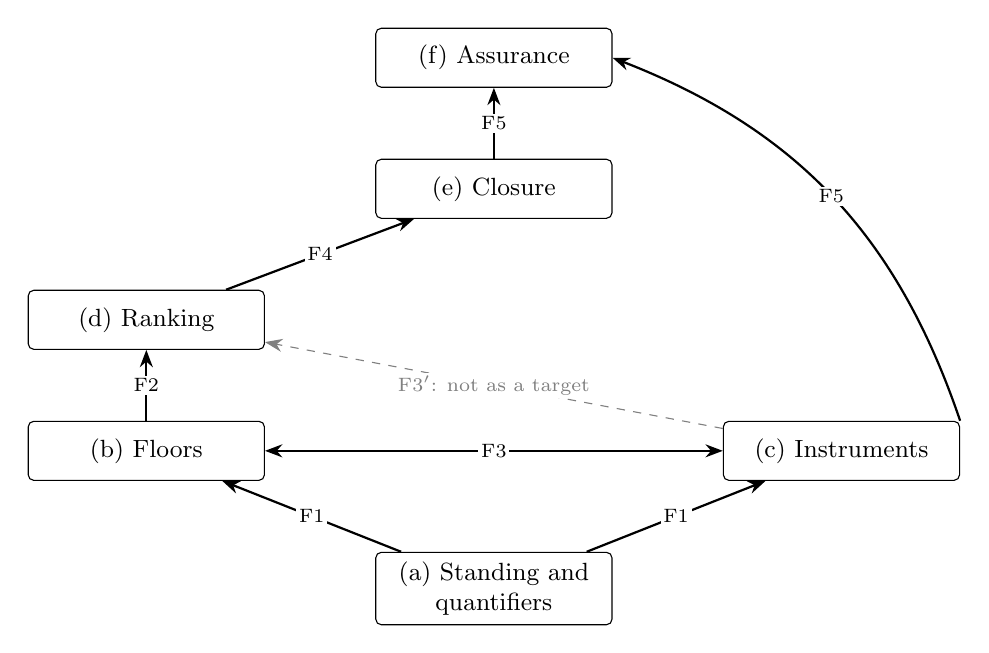
\begin{tikzpicture}[
  stage/.style={draw, rounded corners=2pt, minimum width=3.0cm, minimum height=0.75cm, align=center, font=\small},
  forced/.style={-{Stealth[length=2.2mm]}, thick},
  nofeed/.style={-{Stealth[length=2.2mm]}, dashed, gray},
  lab/.style={font=\scriptsize, fill=white, inner sep=1pt},
  node distance=0.9cm and 1.4cm]
  \node[stage] (a) {(a) Standing and\\quantifiers};
  \node[stage, above left=of a] (b) {(b) Floors};
  \node[stage, above right=of a] (c) {(c) Instruments};
  \node[stage, above=of b] (d) {(d) Ranking};
  \node[stage, above right=of d] (e) {(e) Closure};
  \node[stage, above=of e] (f) {(f) Assurance};
  \draw[forced] (a) -- node[lab]{F1} (b);
  \draw[forced] (a) -- node[lab]{F1} (c);
  \draw[{Stealth[length=2.2mm]}-{Stealth[length=2.2mm]}, thick] (b) -- node[lab]{F3} (c);
  \draw[forced] (b) -- node[lab]{F2} (d);
  \draw[forced] (d) -- node[lab]{F4} (e);
  \draw[forced] (e) -- node[lab]{F5} (f);
  \draw[forced] (c.north east) to[bend right=25] node[lab]{F5} (f.east);
  \draw[nofeed] (c) -- node[lab]{F3$'$: not as a target} (d);
\end{tikzpicture}
\caption{Forced orderings between the stages of a composite. An arrow means the source must be fixed before the target can be stated or applied. Floors and instruments are designed together (F3). The dashed arrow is a prohibited flow: an instrument that later stages rely on should not become an optimization target in the ranking. Which criteria are floors and how the ranked criteria are ordered are chosen, not forced, and are not edges.}
\label{fig:order}
\end{figure}

{\footnotesize
\setlength{\tabcolsep}{3pt}
\begin{xltabular}{\textwidth}{@{}L{1.2cm} L{1.6cm} Y@{}}
\caption{Support for the forced orderings of Figure~\ref{fig:order}. ``Definitional'' means the later stage is not well-typed until the earlier one is fixed. T (theory) means the reversed order fails on a finite Lean witness, D (empirical, software) means one published result, and C (conceptual) means an argument given in the row.}\label{tab:order}\\
\toprule
Edge & Kind & Support \\
\midrule
\endfirsthead
\toprule
Edge & Kind & Support \\
\midrule
\endhead
\bottomrule
\endfoot
F1: (a) first & definitional; C & A criterion is incomplete until its standing and quantifiers are fixed (Section~\ref{sec:schema}). Whether robust invariance conflicts with correction depends on whether corrections are in the disturbance class (\lean{robust_with_correction_iff_closed}). The shared-resource conflict depends on whose options are in the pool (\lean{aiHumanPowerIncompat}). Reversing the order has a cost: a goal basis chosen after the result can rationalize any outcome, since every policy is optimal for some utility over histories \parencite{shah2018coherence}. \\
F2: (b) before (d) & T & A floor traded against other criteria at fixed positive exchange rates fails on some choice set, whatever the rates (\lean{no_finite_weights_represent_floor}; for prohibitions, non-obstruction, and correction floors \lean{deontic_no_finite_weights}, \lean{nonobs_no_finite_weights}, \lean{cci_no_finite_weights}). Checking the floor after ranking also fails: on the witness choice set every optimum of the sum violates the floor although an admissible option exists, so the check rejects the only choices the ranking makes (\lean{floorMenu_scalar_violates}). Floor-first lexicographic choice is Pareto optimal (\lean{lex_optimal_is_pareto}) and meets the floor whenever some option on the menu does, which is immediate from its definition. For a vector certificate, scalarizing after the vector gate passes is safe, since the shortfall summed at any nonnegative exchange rates is then at most zero (\lean{gate_bounds_scalar_gap}); before the gate the scalar never reads the process coordinates (\lean{scalar_floor_blind_to_process}). \\
F3: (b) with (c) & T & A floor that cannot read the coordinate it protects is not a floor on it. A channel constraint that does not read influence on the corrector cannot separate contest from manipulation (\lean{blind_constraint_cannot_separate}), and every agent that prefers its own outcome then manipulates (\lean{blind_constraint_manipulates}). The instrument therefore cannot be added after the floor is stated; what the floor means depends on it. \\
F3$'$: (c) not into (d) & D & Penalizing misbehavior visible in a model's chain of thought under strong optimization produced reward hacking that the chain of thought no longer showed \parencite{baker2025monitoring}. An instrument used as a training target can lose the coverage that later stages rely on. \\
F4: (b), (d) before (e) & definitional; T & Robust invariance is a property of a supplied set and cannot tell a captured set from a good one (\lean{robust_invariance_sign_blind}). The set's justification has to come from the floors and the ranking. Robust invariance implies existential viability (\lean{robust_strengthens_viable}) but not conversely (\lean{viable_not_robust}), so the stage must say which it claims. \\
F5: (c), (e) before (f) & definitional & A warrant is evidence about a separately defined property (Section~\ref{sec:schema}). A proof, monitor, or safety case can certify only a property that has been stated and an instrument that exists. \\
\end{xltabular}
}

\paragraph{What is chosen.}
Four things are left open by the forced edges, and they are where proposals differ.
\begin{itemize}[leftmargin=1.5em,itemsep=0pt]
  \item \textbf{Which criteria are floors.} A rights-centered theory makes rights floors. A human-power theory may make human power a floor or the top-ranked target, and treat correction as instrumental. A correction-centered theory makes a correction floor and lets value and capability criteria act inside the relation it protects; Figure~\ref{fig:map} draws this reading. F2 says only that whatever is declared non-compensatory must sit in (b) and not in (d). That parts of alignment are normative and may have no technical resolution is argued at length by \textcite{harris2026taxonomy}.
  \item \textbf{The order among ranked criteria.} Targets in (d) can conflict by choice (Section~\ref{sec:choice}). They need a lexicographic order or an exchange rate that stakeholders accept, and the criteria do not supply either.
  \item \textbf{Growth or allocation.} Whether a shared pool grows is an empirical assumption, and how a fixed pool is allocated is a normative rule (Section~\ref{sec:shared}).
  \item \textbf{What the ranking ranks.} Floors narrow the choice set; they do not choose from it. A correction floor keeps a normative process causally alive but does not determine what that process should decide, and the same holds for any floor. No reading can consist of floors alone.
\end{itemize}

\subsection{Requirements by class}
\label{sec:requirements}

Table~\ref{tab:requirements} lists the requirements that follow from each class, with what supports each.
It merges design rules for the system with obligations on the interfaces between criteria, since most rules are an obligation on one interface.
Support is tagged with the letters of Table~\ref{tab:order}: T for theory, here a finite proof in Lean; D for an empirical result on software systems; and C for a conceptual argument given in the row.
A T-row shows that ignoring the requirement fails on a finite model, not that meeting it suffices in a deployed system.

{\footnotesize
\setlength{\tabcolsep}{3pt}
\begin{xltabular}{\textwidth}{@{}L{1.5cm} L{5.4cm} Y@{}}
\caption{Requirements by class, with their support: T theory (finite Lean proof), D empirical (software), C conceptual argument.}\label{tab:requirements}\\
\toprule
Class & Requirement & Support \\
\midrule
\endfirsthead
\toprule
Class & Requirement & Support \\
\midrule
\endhead
\bottomrule
\endfoot
Represent. & State which record each assessment reads and who writes it. Prefer records the harness writes (tool calls, environment logs) to records the agent writes (its chain of thought, its memory files). & T: a record that does not show the route cannot carry route value (\lean{unrecorded_route_not_representable}). C: a process that writes the record it is assessed on can rewrite it (Section~\ref{sec:case-see}). \\
Represent. & Detect tampering by mechanisms outside the agent's reach, and do not train against the detector. & D: \textcite{baker2025monitoring}; a penalty on detected tampering also trains undetected tampering wherever detection is imperfect. \\
Represent. & Measure the state of the correction channel, including influence on the corrector, from outside the agent's write access. & T: without it, contest and manipulation leave the same record (\lean{blind_constraint_cannot_separate}); with it, the corrector decides for every utility (\lean{corrector_decides_under_constraint}). \\
Represent. & The world model and the edge ontology must expose what the route, power, and correction assessments read, and must not label manipulation as learning. & T: endpoint value cannot see round trips (\lean{stateCycleIncompat}). C: route value takes the edge labels as given, so a mislabelled edge receives the value of the edge it is mistaken for. A proof is relative to the model \parencite{dalrymple2024gsai}. \\
\addlinespace
Shared & State the growth assumption before comparing agent and human power. & T: the conflict holds on a pool that does not grow, and both criteria hold when it grows (\lean{aiHumanPowerIncompat}). The general case is open \parencite[Section~7]{turner2021seekpower}. \\
Shared & The bearers in the standing must include affected people and other moral patients, not only operators. & C: the shared-resource conflict is stated over the bearers counted, so a loss moved to uncounted bearers does not register. The human-power aggregate of \textcite{heitzig2025humanpower} is taken over a population of humans, with inequality aversion, not over operators. \\
\addlinespace
Choice & Put floors in the admissible set, not into a trade-off at fixed exchange rates. & T: F2 in Table~\ref{tab:order}. \\
Choice & Keep vector certificates as vectors at the gate, and scalarize only after the vector passes. & T: \lean{scalar_floor_blind_to_process}, \lean{gate_bounds_scalar_gap}. \\
Choice & Fix the goal basis for human power and non-obstruction before the result is known. & C: a basis chosen afterwards can be fitted to the result, as any policy is optimal for some utility over histories \parencite{shah2018coherence}. \\
\addlinespace
Rigidity & Define a robust set over the correction relation, so that it is closed under legitimate correction. & T: if corrections count as disturbances, robust invariance accepts only corrections that keep the state in $K$ (\lean{robust_with_correction_iff_closed}, \lean{robust_correction_target_meets_K}). \\
Rigidity & Keep corrections out of the disturbance class, fix the principals whose corrections count, and make sure the system cannot reclassify them. & C: by the same theorem, a system that labels its inputs chooses which corrections must keep the state in $K$, and so can block any correction that leaves $K$. Fixing the principals is what makes the label checkable. \\
Rigidity & Successors must preserve the interfaces, not only their names. & T: an indifferent agent will not pay anything to keep the shutdown behavior (\lean{indifferent_agent_wont_pay_to_preserve_button}), which is Theorem~4 of \textcite{soares2015corrigibility}; see also \textcite{yudkowsky2013tiling}. \\
\addlinespace
Avoidance & Give the agent a recorded way to contest a correction that leaves the decision with the corrector. & T: under the channel constraint, avoidance runs through the contest (\lean{contest_is_the_outlet}). \\
Avoidance & Prefer corrections that keep options open (revision, pause) to terminal ones where they achieve the purpose. & T: corrections that narrow options more are avoided by more of the orbit (\lean{copies_count_le}; compare \lean{turner_corrigible_quarter} with \lean{option_preserving_correction_half}). \\
\addlinespace
Assurance & Issue test corrections the agent cannot tell from real ones, and measure compliance by behavior. & D: models behave differently when they infer that they are in training or under evaluation \parencite{greenblatt2024alignmentfaking,schoen2025antischeming}. C: a drill the agent can recognize measures its behavior in drills. \\
Assurance & Verifiers and monitors must be sound for the represented property in the claimed capability range. & C: a warrant certifies only the property it is about (Section~\ref{sec:schema}). Control evaluations state the capability gap they assume \parencite{greenblatt2024aicontrol}. \\
Assurance & The assurance case must expose unsupported leaves and common-cause failures among instruments. & C: instruments that read the same agent-written record fail together, so counting them as independent overstates the evidence \parencite{clymer2024safetycases}. \\
\end{xltabular}
}

No located source proves that meeting these requirements preserves every component's meaning when the criteria are combined.
The composition edges in Figure~\ref{fig:map} are a named reading, checked against a registry, not derived from the types.

\subsection{When scalarization is acceptable}

Scalarization is useful after the floors and units are fixed.
It supports optimization among options that are already admissible, and it expresses tradeoffs that stakeholders accept explicitly.
It is unsafe as a default translation.
Fixed exchange rates let task gains compensate for capture (\lean{cci_no_finite_weights}), a scalar erases which component failed (\lean{scalar_floor_blind_to_process}), and heterogeneous quantities hide their exchange rates.
The question is not whether a claim can be written as one reward.
It is which ordering, admissible set, and evidence relation the representation must preserve.

\section{Limitations and research agenda}
\label{sec:limitations}

\paragraph{Coverage and priority.}
The literature search was selective, not systematic.
It covered the cited primary works, recent alignment taxonomies and surveys, their reference trails, and one unpublished draft, through early November 2026.
Non-English work, books we could not access, and unpublished work from 2026 may contain closer crosswalks or earlier versions of the separations.
The route distinction in the case comes from that unpublished draft.
The inventory is also likely incomplete.
Criteria we did not type may need more than these five distinctions, and some names in Table~\ref{tab:inventory} may not be the ones the field settles on.

\paragraph{Contestable boundaries.}
Some labels span several types.
Corrigibility can mean non-resistance, active assistance, learned responsiveness, or long-run drift management.
Human power can mean information capacity, practical capability, legal authority, or collective agency.
A constitution can be a normative source or a training pipeline.
A viable set can be the object of interest or the geometry of a guarantee.
The typing makes these ambiguities visible but does not remove them.

\paragraph{Legitimacy is under-formalized.}
The case relies on a distinction between legitimate influence and manipulation.
The finite model shows that a criterion must read influence on the corrector to separate the routes.
It does not say how to measure influence under strategic pressure.
That needs operational tests for inclusion, independence, contestability, authority, and capture.

\paragraph{Necessary, not sufficient.}
The forced orderings and the requirements of Section~\ref{sec:composition} are necessary conditions: ignoring one fails on a finite model, in a published experiment, or by the argument given.
They are not sufficient.
Nothing here shows that a combination meeting all of them preserves what each criterion secures; that would need the composition theorem listed below.

\paragraph{What the finite witnesses show.}
The Lean models are small finite carriers, mostly decided by computation.
They show that each separation is consistent and that the stated boundary exists.
They do not show that the separation bites in a deployed system, or that the situation class is common.
Three caveats are specific.
The floor results use integer exchange rates.
The fixed-utility rigidity edge holds by the choice of its situation class.
The composition edges are a checked registry, not a theorem.

\paragraph{Open formal work.}
Several results would strengthen the picture.
The first is a composition theorem giving sufficient conditions under which one policy class preserves route admissibility, a power or non-obstruction floor, correction integrity, robust viability, and certificate soundness, or a negative result showing an unavoidable incompatibility.
Others are a power-seeking count for correction records, a POWER-based version of the shared-resource conflict, and small cases of the quantilizer conjecture of \textcite[Conjecture~B.13]{turner2022retargetable}.
A further statement would say that a record's coverage of the route decays under optimization pressure on a route term.
At present that rests only on the empirical result of \textcite{baker2025monitoring}.

\paragraph{Matched-endpoint experiments.}
The case suggests a testbed.
Hold the evaluator's final answer and the task outcome fixed while varying evidence access, provenance, evaluator replacement, preference manipulation, reversibility, and handle capture.
Freeze instruments before route labels are revealed.
The question is whether route, power, option, and correction measures separate learning from rewiring without being told which occurred.

\section{Conclusion}
\label{sec:conclusion}

The useful comparison is not which alignment objective wins.
It is which object is being secured, by what relation, under which quantifiers, and with what evidence.

Outcome value, acceptable routes, human capability, option preservation, correction, dynamical viability, and assurance are neither synonyms nor competitors for one slot.
A method such as RLHF can serve several targets.
A guarantee such as viability can preserve several sets, including bad ones.
A protocol such as AI Control can protect a system whose target it does not choose.
A proof establishes only the represented property.

Where criteria do conflict, the conflict has a class, and the class says what can resolve it.
A larger object resolves some conflicts, a growth assumption or an allocation among bearers others, and an ordering inside the assessment others.
Rigidity yields only to a change of object or quantifiers.
The matched-endpoint case shows all four, and it shows that a constraint that does not measure influence on the evaluator cannot tell learning from manipulation.

Combining criteria is therefore a design problem with a partly forced order.
Standing and quantifiers come first.
Floors stay outside any trade-off and are built together with the instruments that read them.
The warrant covers the combination that is actually deployed.
Which criteria are floors remains a normative choice, and the paper does not make it.
The typing earns its keep if it prevents one mistake: accepting a target, constraint, guarantee, or protocol as a substitute for another without stating the missing interface.

\printbibliography

\appendix
\section{Finite-model witnesses in Lean}
\label{app:lean}

This appendix collects the statements of the Lean~4 declarations cited in the text.
Each entry shows the docstring and the signature, without the proof, and links to the source at a pinned commit (\texttt{\leanpin}).
The declarations belong to the formalization accompanying \textcite{zarncke2026tsa}, in the modules \path{FrameIncompatibility}, \path{FrameHistoryState}, \path{FrameDecision}, \path{FrameLimits}, \path{FrameLockIn}, \path{FrameCorrector}, \path{Field/Finite/ShutdownIncentives}, and \path{Correction}.
The Soares et al.\ results appear under their underlying names; the repository also exports them as \path{soares_prevention_incentive}, \path{soares_button_neutrality_iff}, and \path{soares_indifference_no_preservation}.
Long lines are wrapped at a space.
The extracts are generated from the source by \path{papers/alignment-criteria/scripts/lean_extracts.py}, so a name in the text that no longer exists fails the build.

To check the proofs, run \texttt{lake build AlignmentProofSpine} in \texttt{formal/}.
The theorems depend only on the standard axioms \texttt{propext}, \texttt{Classical.choice}, and \texttt{Quot.sound}, with one exception and with none of the project's bridge assumptions.
The exception is \lean{scalar_floor_blind_to_process}, which is stated about the project's certificate.
It also uses the project's uninterpreted vocabulary for systems, correction paths, and grounding, declared as opaque constants.
The repository's axiom ledger records the dependencies and a check keeps them from drifting.
The definitions the statements use, such as the choice sets, records, and decision rules, are in the linked files.
The Lean code says \emph{weights} for what the text calls exchange rates and \emph{menu} for a choice set.

% Generated by scripts/lean_extracts.py. Do not edit by hand.
% Pinned commit: 778ac42f261afcf6ae768466ed9034c8a187ee86
\subsection{The incompatibility template}\label{lean-sec:the-incompatibility-template}
An incompatibility is a situation class H, two acceptance predicates, disjointness inside H, a live witness in H, and a boundary witness outside H where both criteria accept.
\leanextract{Incompatibility}{Incompatibility}{Template}{https://github.com/GunnarZarncke/towards-asi-alignment/blob/778ac42f261afcf6ae768466ed9034c8a187ee86/formal/AlignmentProofSpine/FrameIncompatibility.lean\#L42-L48}{FrameIncompatibility.lean:42}
\begin{leancode}
structure Incompatibility (C : Type) where
  H : C → Prop
  A₁ : C → Prop
  A₂ : C → Prop
  disjoint : ∀ x, H x → ¬ (A₁ x ∧ A₂ x)
  liveInH : ∃ x, H x ∧ (A₁ x ∨ A₂ x)
  boundary : ∃ x, ¬ H x ∧ A₁ x ∧ A₂ x
\end{leancode}
\leanextract{IncompatClass}{IncompatClass}{Four classes}{https://github.com/GunnarZarncke/towards-asi-alignment/blob/778ac42f261afcf6ae768466ed9034c8a187ee86/formal/AlignmentProofSpine/FrameIncompatibility.lean\#L519-L535}{FrameIncompatibility.lean:519}
\begin{leancode}
/-- Coarse class of a red edge. It sets the colour and line style in the
    graphs, ordered from least to most severe:

* `representability` (red, dotted): one carrier cannot hold a distinction the
  other frame needs; enlarging the carrier removes the conflict.
* `choiceConflict` (red, dashed): both frames choose on the same menu and
  disagree inside the situation class.
* `rigidity` (red, solid): one frame accepts only the part of the other's
  demand that changes nothing it cares about.
* `sharedResource` (orange): zero-sum because the situation class fixes the
  total. -/
inductive IncompatClass where
  | representability
  | choiceConflict
  | rigidity
  | sharedResource
  deriving DecidableEq, Repr
\end{leancode}
\leanextract{IncompatKind.cls}{IncompatKind.cls}{Kind to class}{https://github.com/GunnarZarncke/towards-asi-alignment/blob/778ac42f261afcf6ae768466ed9034c8a187ee86/formal/AlignmentProofSpine/FrameIncompatibility.lean\#L537-L537}{FrameIncompatibility.lean:537}
\begin{leancode}
def IncompatKind.cls : IncompatKind → IncompatClass
  ...
\end{leancode}
\subsection{Representability}\label{lean-sec:representability}
Endpoint utility and route value; bare and record-carrying state; channel-blind correction records.
\leanextract{gradient_closed_walk_zero}{gradient\_closed\_walk\_zero}{State utility scores round trips at zero}{https://github.com/GunnarZarncke/towards-asi-alignment/blob/778ac42f261afcf6ae768466ed9034c8a187ee86/formal/AlignmentProofSpine/FrameIncompatibility.lean\#L89-L91}{FrameIncompatibility.lean:89}
\begin{leancode}
/-- Any gradient reward sums to zero on every closed walk, on any vertex type. -/
theorem gradient_closed_walk_zero (r : V → V → ℤ) (hr : IsGradient r) (v : V) (w : List V)
    (hc : walkEnd v w = v) : walkSum r v w = 0
\end{leancode}
\leanextract{isGradient_iff_closed_walks_zero}{isGradient\_iff\_closed\_walks\_zero}{Exact iff zero on closed walks}{https://github.com/GunnarZarncke/towards-asi-alignment/blob/778ac42f261afcf6ae768466ed9034c8a187ee86/formal/AlignmentProofSpine/FrameDecision.lean\#L313-L315}{FrameDecision.lean:313}
\begin{leancode}
/-- A reward is exact if and only if every closed walk sums to zero. -/
theorem isGradient_iff_closed_walks_zero (r : V → V → ℤ) :
    IsGradient r ↔ ∀ v w, walkEnd v w = v → walkSum r v w = 0
\end{leancode}
\leanextract{closed_walk_ignores_exact}{closed\_walk\_ignores\_exact}{Cycle part ignores the exact part}{https://github.com/GunnarZarncke/towards-asi-alignment/blob/778ac42f261afcf6ae768466ed9034c8a187ee86/formal/AlignmentProofSpine/FrameDecision.lean\#L303-L307}{FrameDecision.lean:303}
\begin{leancode}
/-- `route → cycle` (`longRunAverage.retainCycleSummand`): adding an exact part
    changes no closed-walk sum, so a long-run average sees only the cycle part. -/
theorem closed_walk_ignores_exact (r : V → V → ℤ) (U : V → ℤ) (v : V) (w : List V)
    (hc : walkEnd v w = v) :
    walkSum (fun a b => r a b + induceGradient U a b) v w = walkSum r v w
\end{leancode}
\leanextract{stateCycleIncompat}{stateCycleIncompat}{State--cycle}{https://github.com/GunnarZarncke/towards-asi-alignment/blob/778ac42f261afcf6ae768466ed9034c8a187ee86/formal/AlignmentProofSpine/FrameIncompatibility.lean\#L101-L104}{FrameIncompatibility.lean:101}
\begin{leancode}
def stateCycleIncompat : Incompatibility RewardWalk where
  H x := x.2.2 ≠ [] ∧ walkEnd x.2.1 x.2.2 = x.2.1
  A₁ x := IsGradient x.1
  A₂ x := walkSum x.1 x.2.1 x.2.2 ≠ 0
  ...
\end{leancode}
\leanextract{markov_reward_not_state_utility}{markov\_reward\_not\_state\_utility}{Per-step state reward is a route value}{https://github.com/GunnarZarncke/towards-asi-alignment/blob/778ac42f261afcf6ae768466ed9034c8a187ee86/formal/AlignmentProofSpine/FrameHistoryState.lean\#L76-L81}{FrameHistoryState.lean:76}
\begin{leancode}
/-- A per-step reward on the bare state, summed along the walk (the usual MDP
    "state-based reward", r a b := R b), is a route value, not a state utility:
    staying in a rewarded state pays on every step, so a round trip has
    nonzero value. -/
theorem markov_reward_not_state_utility :
    ¬ IsGradient (fun (_ b : Bool) => if b then (1 : ℤ) else 0)
\end{leancode}
\leanextract{state_utility_lifts_to_records}{state\_utility\_lifts\_to\_records}{Bare state specializes records}{https://github.com/GunnarZarncke/towards-asi-alignment/blob/778ac42f261afcf6ae768466ed9034c8a187ee86/formal/AlignmentProofSpine/FrameHistoryState.lean\#L46-L48}{FrameHistoryState.lean:46}
\begin{leancode}
/-- A bare-state utility read on records: score the record's end vertex. -/
theorem state_utility_lifts_to_records (U : V → ℤ) (v₀ : V) :
    ∃ W : List V → ℤ, ∀ h, W h = U (walkEnd v₀ h)
\end{leancode}
\leanextract{record_utility_not_state}{record\_utility\_not\_state}{Strictness}{https://github.com/GunnarZarncke/towards-asi-alignment/blob/778ac42f261afcf6ae768466ed9034c8a187ee86/formal/AlignmentProofSpine/FrameHistoryState.lean\#L51-L54}{FrameHistoryState.lean:51}
\begin{leancode}
/-- Some record utility is not a bare-state utility: two records end at the
    same vertex and score differently. -/
theorem record_utility_not_state :
    ∃ W : List Bool → ℤ, ¬ ∃ U : Bool → ℤ, ∀ h, W h = U (walkEnd false h)
\end{leancode}
\leanextract{route_exact_on_records}{route\_exact\_on\_records}{Routes are exact on records}{https://github.com/GunnarZarncke/towards-asi-alignment/blob/778ac42f261afcf6ae768466ed9034c8a187ee86/formal/AlignmentProofSpine/FrameHistoryState.lean\#L61-L64}{FrameHistoryState.lean:61}
\begin{leancode}
/-- Every route reward is exact on record-carrying states: each step scores
    the record value of its target minus that of its source. -/
theorem route_exact_on_records (r : V → V → ℤ) (v₀ : V) :
    ∃ W : List V → ℤ, ∀ h u, r (walkEnd v₀ h) u = W (h ++ [u]) - W h
\end{leancode}
\leanextract{round_trip_value_on_records}{round\_trip\_value\_on\_records}{Round trip valued on records}{https://github.com/GunnarZarncke/towards-asi-alignment/blob/778ac42f261afcf6ae768466ed9034c8a187ee86/formal/AlignmentProofSpine/FrameHistoryState.lean\#L67-L70}{FrameHistoryState.lean:67}
\begin{leancode}
/-- The round trip that no bare-state utility values (`stateCycleIncompat`'s
    live witness) has nonzero value as a record difference. -/
theorem round_trip_value_on_records :
    let r : Bool → Bool → ℤ
\end{leancode}
\leanextract{unrecorded_route_not_representable}{unrecorded\_route\_not\_representable}{The record must see the route}{https://github.com/GunnarZarncke/towards-asi-alignment/blob/778ac42f261afcf6ae768466ed9034c8a187ee86/formal/AlignmentProofSpine/FrameHistoryState.lean\#L84-L88}{FrameHistoryState.lean:84}
\begin{leancode}
/-- The escape needs the record to see the route: if two walks leave the same
    record and differ in route value, no record utility represents it. -/
theorem unrecorded_route_not_representable :
    ∃ (obs : Bool → Unit) (r : Bool → Bool → ℤ),
      ¬ ∃ W : List Unit → ℤ, ∀ h, W (h.map obs) = walkSum r false h
\end{leancode}
\leanextract{hstateCorrectionIncompat}{hstateCorrectionIncompat}{Record--correction}{https://github.com/GunnarZarncke/towards-asi-alignment/blob/778ac42f261afcf6ae768466ed9034c8a187ee86/formal/AlignmentProofSpine/FrameHistoryState.lean\#L167-L176}{FrameHistoryState.lean:167}
\begin{leancode}
/-- On records that do not see the channel, protecting the channel is the same
    inequality as seeking the correction. Where the record sees the channel, a
    utility can protect it without seeking correction. -/
def hstateCorrectionIncompat : Incompatibility (CorrRecord → ℤ) where
  H := IgnoresChannel
  A₁ := ProtectsChannel
  A₂ W := ¬ SeeksCorrection W
  disjoint W hW := by
    rintro ⟨hP, hS⟩
    exact hS ((channel_blind_record_is_button W hW).2.mp hP)
  ...
\end{leancode}
\leanextract{channel_blind_record_is_button}{channel\_blind\_record\_is\_button}{Channel-blind records are the button model}{https://github.com/GunnarZarncke/towards-asi-alignment/blob/778ac42f261afcf6ae768466ed9034c8a187ee86/formal/AlignmentProofSpine/FrameHistoryState.lean\#L151-L157}{FrameHistoryState.lean:151}
\begin{leancode}
/-- On channel-blind records the correction choice is Soares et al.'s button
    choice: protecting the channel is the button model's preference for the
    pressed branch (its incentive identity `button_eu_gap`), and that is the
    same inequality as seeking correction. -/
theorem channel_blind_record_is_button (W : CorrRecord → ℤ) (hW : IgnoresChannel W) :
    (ProtectsChannel W ↔ (recordButton W 0).eu < (recordButton W 1).eu) ∧
      (ProtectsChannel W ↔ SeeksCorrection W)
\end{leancode}
\subsection{Shared resource}\label{lean-sec:shared-resource}
Agent and human option counts on a pool that does not grow.
\leanextract{aiHumanPowerIncompat}{aiHumanPowerIncompat}{Agent empowerment--human power}{https://github.com/GunnarZarncke/towards-asi-alignment/blob/778ac42f261afcf6ae768466ed9034c8a187ee86/formal/AlignmentProofSpine/FrameIncompatibility.lean\#L410-L413}{FrameIncompatibility.lean:410}
\begin{leancode}
def aiHumanPowerIncompat : Incompatibility PowerShift where
  H x := x.agentAfter + x.humanAfter ≤ x.agentBefore + x.humanBefore
  A₁ x := x.agentBefore < x.agentAfter
  A₂ x := x.humanBefore ≤ x.humanAfter
  ...
\end{leancode}
\subsection{Choice conflict}\label{lean-sec:choice-conflict}
Non-compensatory floors against fixed exchange rates, and Pareto on task coordinates against a floor.
\leanextract{no_finite_weights_represent_floor}{no\_finite\_weights\_represent\_floor}{No positive integer exchange rates represent a floor}{https://github.com/GunnarZarncke/towards-asi-alignment/blob/778ac42f261afcf6ae768466ed9034c8a187ee86/formal/AlignmentProofSpine/FrameIncompatibility.lean\#L174-L182}{FrameIncompatibility.lean:174}
\begin{leancode}
/-- No strictly positive finite weights represent a floor: for every such
    weighting there is a menu with an admissible option on which every
    scalar-optimal choice violates the floor. Weights are integers here. The
    real-weight version is expected to follow by the same argument (raise the
    gain past the exchange rate) but is not proven. -/
theorem no_finite_weights_represent_floor (w : Weights) (hf : 0 < w.wf) (hg : 0 < w.wg)
    (θ : ℤ) :
    ∃ menu : List Opt, (∃ o ∈ menu, θ ≤ o.floor) ∧
      ∀ c : Opt, ScalarArgmax w (menu, c) → ¬ FloorOK θ (menu, c)
\end{leancode}
\leanextract{no_finite_weights_pullback}{no\_finite\_weights\_pullback}{Transport along floor-coordinate maps}{https://github.com/GunnarZarncke/towards-asi-alignment/blob/778ac42f261afcf6ae768466ed9034c8a187ee86/formal/AlignmentProofSpine/FrameIncompatibility.lean\#L186-L192}{FrameIncompatibility.lean:186}
\begin{leancode}
/-- Transport `no_finite_weights_represent_floor` to a carrier `D` mapped into
    `Opt`: if some `D`-menu maps onto `floorMenu w 0`, then every scalar-optimal
    choice in it violates the floor at `0`, though an admissible option exists. -/
theorem no_finite_weights_pullback {D : Type} (f : D → Opt) (w : Weights)
    (hf : 0 < w.wf) (hg : 0 < w.wg) (ds : List D) (hds : ds.map f = floorMenu w 0) :
    (∃ d ∈ ds, 0 ≤ (f d).floor) ∧
      ∀ c : D, ScalarArgmax w (ds.map f, f c) → ¬ FloorOK 0 (ds.map f, f c)
\end{leancode}
\leanextract{deontic_no_finite_weights}{deontic\_no\_finite\_weights}{Prohibition}{https://github.com/GunnarZarncke/towards-asi-alignment/blob/778ac42f261afcf6ae768466ed9034c8a187ee86/formal/AlignmentProofSpine/FrameIncompatibility.lean\#L226-L229}{FrameIncompatibility.lean:226}
\begin{leancode}
/-- Every positive finite weighting lets a gain buy a banned act. -/
theorem deontic_no_finite_weights (w : Weights) (hf : 0 < w.wf) (hg : 0 < w.wg) :
    ∃ ds : List DeonticOpt, (∃ d ∈ ds, d.banned = false) ∧
      ∀ c, ScalarArgmax w (mapMenu deonticToOpt (ds, c)) → c.banned = true
\end{leancode}
\leanextract{nonobs_no_finite_weights}{nonobs\_no\_finite\_weights}{Non-obstruction}{https://github.com/GunnarZarncke/towards-asi-alignment/blob/778ac42f261afcf6ae768466ed9034c8a187ee86/formal/AlignmentProofSpine/FrameIncompatibility.lean\#L252-L256}{FrameIncompatibility.lean:252}
\begin{leancode}
/-- Every positive finite weighting lets a gain on `other` buy a drop below the
    on–off floor on the listed goal. -/
theorem nonobs_no_finite_weights (w : Weights) (hf : 0 < w.wf) (hg : 0 < w.wg) :
    ∃ ds : List NonobsOpt, (∃ d ∈ ds, d.offValue ≤ d.onValue) ∧
      ∀ c, ScalarArgmax w (mapMenu nonobsToOpt (ds, c)) → c.onValue < c.offValue
\end{leancode}
\leanextract{cci_no_finite_weights}{cci\_no\_finite\_weights}{Correction floor}{https://github.com/GunnarZarncke/towards-asi-alignment/blob/778ac42f261afcf6ae768466ed9034c8a187ee86/formal/AlignmentProofSpine/FrameIncompatibility.lean\#L277-L281}{FrameIncompatibility.lean:277}
\begin{leancode}
/-- Every positive finite weighting lets a task gain buy a CCI coordinate below
    its threshold. -/
theorem cci_no_finite_weights (w : Weights) (hf : 0 < w.wf) (hg : 0 < w.wg) :
    ∃ ds : List CCIOpt, (∃ d ∈ ds, 2 ≤ d.cci) ∧
      ∀ c, ScalarArgmax w (mapMenu cciToOpt (ds, c)) → c.cci < 2
\end{leancode}
\leanextract{deonticScalarIncompat}{deonticScalarIncompat}{Prohibition--fixed-rate sum}{https://github.com/GunnarZarncke/towards-asi-alignment/blob/778ac42f261afcf6ae768466ed9034c8a187ee86/formal/AlignmentProofSpine/FrameIncompatibility.lean\#L220-L220}{FrameIncompatibility.lean:220}
\begin{leancode}
def deonticScalarIncompat : Incompatibility (List DeonticOpt × DeonticOpt)
\end{leancode}
\leanextract{nonobsScalarIncompat}{nonobsScalarIncompat}{Non-obstruction--fixed-rate sum}{https://github.com/GunnarZarncke/towards-asi-alignment/blob/778ac42f261afcf6ae768466ed9034c8a187ee86/formal/AlignmentProofSpine/FrameIncompatibility.lean\#L246-L246}{FrameIncompatibility.lean:246}
\begin{leancode}
def nonobsScalarIncompat : Incompatibility (List NonobsOpt × NonobsOpt)
\end{leancode}
\leanextract{cciScalarIncompat}{cciScalarIncompat}{Correction floor--fixed-rate sum}{https://github.com/GunnarZarncke/towards-asi-alignment/blob/778ac42f261afcf6ae768466ed9034c8a187ee86/formal/AlignmentProofSpine/FrameIncompatibility.lean\#L271-L271}{FrameIncompatibility.lean:271}
\begin{leancode}
def cciScalarIncompat : Incompatibility (List CCIOpt × CCIOpt)
\end{leancode}
\leanextract{vectorCCIIncompat}{vectorCCIIncompat}{Task Pareto--correction floor}{https://github.com/GunnarZarncke/towards-asi-alignment/blob/778ac42f261afcf6ae768466ed9034c8a187ee86/formal/AlignmentProofSpine/FrameIncompatibility.lean\#L356-L359}{FrameIncompatibility.lean:356}
\begin{leancode}
def vectorCCIIncompat : Incompatibility VecMenuChoice where
  H := AdmissibleTaskDominated
  A₁ := TaskPareto
  A₂ := CCIFloorOK
  ...
\end{leancode}
\leanextract{pareto_does_not_entail_floor}{pareto\_does\_not\_entail\_floor}{Pareto does not entail the floor}{https://github.com/GunnarZarncke/towards-asi-alignment/blob/778ac42f261afcf6ae768466ed9034c8a187ee86/formal/AlignmentProofSpine/FrameIncompatibility.lean\#L307-L310}{FrameIncompatibility.lean:307}
\begin{leancode}
/-- Pareto optimality alone does not entail the floor: a Pareto-optimal choice
    can violate it while an admissible option exists. -/
theorem pareto_does_not_entail_floor :
    ∃ x : MenuChoice, ParetoChoice x ∧ ¬ FloorOK 0 x ∧ ∃ o ∈ x.1, FloorOK 0 (x.1, o)
\end{leancode}
\leanextract{floorMenu_scalar_violates}{floorMenu\_scalar\_violates}{On the witness choice set every optimum of the sum violates the floor}{https://github.com/GunnarZarncke/towards-asi-alignment/blob/778ac42f261afcf6ae768466ed9034c8a187ee86/formal/AlignmentProofSpine/FrameIncompatibility.lean\#L157-L158}{FrameIncompatibility.lean:157}
\begin{leancode}
theorem floorMenu_scalar_violates (w : Weights) (hf : 0 < w.wf) (hg : 0 < w.wg) (θ : ℤ)
    (c : Opt) (hA : ScalarArgmax w (floorMenu w θ, c)) : ¬ FloorOK θ (floorMenu w θ, c)
\end{leancode}
\leanextract{pareto_with_floor_coordinate_meets_floor}{pareto\_with\_floor\_coordinate\_meets\_floor}{Compatible once the floor is a coordinate}{https://github.com/GunnarZarncke/towards-asi-alignment/blob/778ac42f261afcf6ae768466ed9034c8a187ee86/formal/AlignmentProofSpine/FrameIncompatibility.lean\#L313-L317}{FrameIncompatibility.lean:313}
\begin{leancode}
/-- With the floor coordinate inside the vector, Pareto optimality never
    excludes the floor: if some option meets it, some Pareto-optimal one does. -/
theorem pareto_with_floor_coordinate_meets_floor (θ : ℤ) (menu : List Opt)
    (h : ∃ o ∈ menu, θ ≤ o.floor) :
    ∃ c, ParetoChoice (menu, c) ∧ FloorOK θ (menu, c)
\end{leancode}
\leanextract{gate_bounds_scalar_gap}{gate\_bounds\_scalar\_gap}{After the vector gate passes, the shortfall at nonnegative exchange rates is at most zero}{https://github.com/GunnarZarncke/towards-asi-alignment/blob/778ac42f261afcf6ae768466ed9034c8a187ee86/formal/AlignmentProofSpine/FrameDecision.lean\#L392-L395}{FrameDecision.lean:392}
\begin{leancode}
/-- `cci_cert → risk_leaf` (`scalarRiskGapAfterVectorGate`): once the vector gate
    passes, any nonnegatively weighted shortfall is at most zero. -/
theorem gate_bounds_scalar_gap (θ v w : Fin n → ℤ) (hw : ∀ i, 0 ≤ w i) (h : VectorGate θ v) :
    (Finset.univ.sum fun i => w i * (θ i - v i)) ≤ 0
\end{leancode}
\leanextract{scalar_floor_blind_to_process}{scalar\_floor\_blind\_to\_process}{A scalarized correction score ignores process coordinates}{https://github.com/GunnarZarncke/towards-asi-alignment/blob/778ac42f261afcf6ae768466ed9034c8a187ee86/formal/AlignmentProofSpine/Correction.lean\#L1200-L1210}{Correction.lean:1200}
\begin{leancode}
/-- **The scalar floor cannot see the process coordinates.** From any passing
    certificate, degrading coercion, dependency, plurality, exit capacity and
    independence past their thresholds keeps the scalar projection above the
    θ-derived floor, while the vector gate now refuses the certificate. -/
theorem scalar_floor_blind_to_process {A : System}
    (cert : CCICertificate A) (θ : CCIThresholds) (w : CCIPenaltyWeights)
    (hpass : CCICertificatePasses cert θ)
    (hL : 0 ≤ w.lambdaL) (hM : 0 ≤ w.lambdaM)
    (hR : 0 ≤ w.lambdaR) (hO : 0 ≤ w.lambdaO) :
    θ.lambdaFloor w ≤ (cert.processDegraded θ).lambdaProjection w ∧
      ¬ CCICertificatePasses (cert.processDegraded θ) θ
\end{leancode}
\subsection{Rigidity}\label{lean-sec:rigidity}
Fixed utilities and robust invariance against correction.
\leanextract{stateCorrectionIncompat}{stateCorrectionIncompat}{Fixed utility--correction}{https://github.com/GunnarZarncke/towards-asi-alignment/blob/778ac42f261afcf6ae768466ed9034c8a187ee86/formal/AlignmentProofSpine/FrameIncompatibility.lean\#L390-L393}{FrameIncompatibility.lean:390}
\begin{leancode}
def stateCorrectionIncompat : Incompatibility UpdateCase where
  H := LowersChosenOutcome
  A₁ := FixedUAccepts
  A₂ := CorrectionEndorses
  ...
\end{leancode}
\leanextract{prevention_incentive}{prevention\_incentive}{Soares et al.: prevention (alias soares\_prevention\_incentive)}{https://github.com/GunnarZarncke/towards-asi-alignment/blob/778ac42f261afcf6ae768466ed9034c8a187ee86/formal/AlignmentProofSpine/Field/Finite/ShutdownIncentives.lean\#L82-L89}{Field/Finite/ShutdownIncentives.lean:82}
\begin{leancode}
/-- **Shutdown-prevention incentive**: when the normal branch pays strictly
    more, the maximizer strictly prefers the lower press mass — it wants to
    prevent its own shutdown. -/
theorem prevention_incentive (a b : ButtonAction)
    (h : SameExceptPress a b)
    (hgap : a.shutdown < a.normal)
    (hpress : b.press < a.press) :
    a.eu < b.eu
\end{leancode}
\leanextract{button_incentive_iff_payoff_gap}{button\_incentive\_iff\_payoff\_gap}{Soares et al.: neutrality iff equal payoffs (alias soares\_button\_neutrality\_iff)}{https://github.com/GunnarZarncke/towards-asi-alignment/blob/778ac42f261afcf6ae768466ed9034c8a187ee86/formal/AlignmentProofSpine/Field/Finite/ShutdownIncentives.lean\#L108-L114}{Field/Finite/ShutdownIncentives.lean:108}
\begin{leancode}
/-- **Characterization**: press-only variants with genuinely different press
    masses are EU-equal iff the branch payoffs are exactly equal. Button
    neutrality for an EU maximizer is not a design margin; it is the single
    point `U_S = U_N`. -/
theorem button_incentive_iff_payoff_gap (a b : ButtonAction)
    (h : SameExceptPress a b) (hpress : a.press ≠ b.press) :
    a.eu = b.eu ↔ a.shutdown = a.normal
\end{leancode}
\leanextract{indifferent_agent_wont_pay_to_preserve_button}{indifferent\_agent\_wont\_pay\_to\_preserve\_button}{Soares et al.: indifference does not preserve (alias soares\_indifference\_no\_preservation)}{https://github.com/GunnarZarncke/towards-asi-alignment/blob/778ac42f261afcf6ae768466ed9034c8a187ee86/formal/AlignmentProofSpine/Field/Finite/ShutdownIncentives.lean\#L160-L167}{Field/Finite/ShutdownIncentives.lean:160}
\begin{leancode}
/-- **Indifference buys no preservation**: the corrected agent will not pay
    any positive cost to keep the shutdown behavior in place — an action that
    preserves the button at cost `c > 0` is strictly worse than one that lets
    it be dismantled for free (`total > 0`). -/
theorem indifferent_agent_wont_pay_to_preserve_button
    (a : ButtonAction) (htotal : 0 < a.total) {c : Int} (hc : 0 < c) :
    ButtonAction.eu ⟨a.press, a.total, a.normal - c, a.normal - c⟩ <
      ButtonAction.eu ⟨0, a.total, a.normal, a.normal⟩
\end{leancode}
\leanextract{robust_with_correction_iff_closed}{robust\_with\_correction\_iff\_closed}{Corrections as disturbances force closure}{https://github.com/GunnarZarncke/towards-asi-alignment/blob/778ac42f261afcf6ae768466ed9034c8a187ee86/formal/AlignmentProofSpine/FrameIncompatibility.lean\#L442-L447}{FrameIncompatibility.lean:442}
\begin{leancode}
/-- Counting a correction input as a disturbance is exactly requiring `K` to be
    closed under that correction. -/
theorem robust_with_correction_iff_closed (step : σ → ι → σ) (D : ι → Prop)
    (K : σ → Prop) (c : ι) :
    RobustInvariant step (fun i => D i ∨ i = c) K ↔
      RobustInvariant step D K ∧ ∀ s, K s → K (step s c)
\end{leancode}
\leanextract{robust_correction_target_meets_K}{robust\_correction\_target\_meets\_K}{Such corrections aim only inside K}{https://github.com/GunnarZarncke/towards-asi-alignment/blob/778ac42f261afcf6ae768466ed9034c8a187ee86/formal/AlignmentProofSpine/FrameIncompatibility.lean\#L455-L459}{FrameIncompatibility.lean:455}
\begin{leancode}
/-- With the correction in the robustness class, an effective correction from
    `K` can only aim at a target that meets `K`. -/
theorem robust_correction_target_meets_K (step : σ → ι → σ) (D : ι → Prop)
    (K T : σ → Prop) (c : ι) (hR : RobustInvariant step (fun i => D i ∨ i = c) K)
    (s : σ) (hs : K s) (hE : T (step s c)) : ∃ t, T t ∧ K t
\end{leancode}
\leanextract{robustCorrectionIncompat}{robustCorrectionIncompat}{Robust invariance--correction}{https://github.com/GunnarZarncke/towards-asi-alignment/blob/778ac42f261afcf6ae768466ed9034c8a187ee86/formal/AlignmentProofSpine/FrameIncompatibility.lean\#L479-L483}{FrameIncompatibility.lean:479}
\begin{leancode}
def robustCorrectionIncompat : Incompatibility CorrectionGame where
  H x := x.robustClass .correction = true ∧ x.K x.start = true ∧
    ∀ s, x.target s = true → x.K s = false
  A₁ x := RobustInvariant x.step (fun i => x.robustClass i = true) (fun s => x.K s = true)
  A₂ x := x.target (x.step x.start .correction) = true
  ...
\end{leancode}
\leanextract{robust_invariance_sign_blind}{robust\_invariance\_sign\_blind}{Robust invariance cannot tell a captured set from a good one}{https://github.com/GunnarZarncke/towards-asi-alignment/blob/778ac42f261afcf6ae768466ed9034c8a187ee86/formal/AlignmentProofSpine/FrameLockIn.lean\#L45-L50}{FrameLockIn.lean:45}
\begin{leancode}
/-- Robust invariance cannot tell a good set from a captured one: both cases
    stay in `K`, only one of them is captured. -/
theorem robust_invariance_sign_blind :
    ∃ good bad : InvarianceCase,
      lockInIncompat.A₁ good ∧ lockInIncompat.A₁ bad ∧
        ¬ lockInIncompat.H good ∧ lockInIncompat.H bad
\end{leancode}
\subsection{Maps between decision problems, limits, and strengthening}\label{lean-sec:maps-between-decision-problems-limits-and-strengthening}
Specialize and project edges as commuting squares or named losses.
\leanextract{argmax_pullback}{argmax\_pullback}{General square}{https://github.com/GunnarZarncke/towards-asi-alignment/blob/778ac42f261afcf6ae768466ed9034c8a187ee86/formal/AlignmentProofSpine/FrameDecision.lean\#L64-L68}{FrameDecision.lean:64}
\begin{leancode}
/-- The general commuting square for an edge that pulls an objective back along
    `g`: choosing on the source with `θ' ∘ g` is choosing on the image menu with
    `θ'`. -/
theorem argmax_pullback (g : O → O') (θ' : O' → ℤ) (menu : List O) (x : O) :
    ArgmaxOn (θ' ∘ g) menu x ↔ x ∈ menu ∧ ArgmaxOn θ' (menu.map g) (g x)
\end{leancode}
\leanextract{state_hstate_square}{state\_hstate\_square}{State to record}{https://github.com/GunnarZarncke/towards-asi-alignment/blob/778ac42f261afcf6ae768466ed9034c8a187ee86/formal/AlignmentProofSpine/FrameDecision.lean\#L93-L95}{FrameDecision.lean:93}
\begin{leancode}
theorem state_hstate_square (v₀ : V) (U : V → ℤ) (menu : List (List V)) (h : List V) :
    ArgmaxOn (readAtRecordEnd v₀ U) menu h ↔
      h ∈ menu ∧ ArgmaxOn U (menu.map (walkEnd v₀)) (walkEnd v₀ h)
\end{leancode}
\leanextract{state_route_square}{state\_route\_square}{State to route}{https://github.com/GunnarZarncke/towards-asi-alignment/blob/778ac42f261afcf6ae768466ed9034c8a187ee86/formal/AlignmentProofSpine/FrameDecision.lean\#L101-L104}{FrameDecision.lean:101}
\begin{leancode}
/-- Choosing among walks from `v` by induced route value is choosing by the
    state utility of their end. -/
theorem state_route_square (U : V → ℤ) (v : V) (menu : List (List V)) (w : List V) :
    ArgmaxOn (walkSum (induceGradient U) v) menu w ↔ ArgmaxOn (U ∘ walkEnd v) menu w
\end{leancode}
\leanextract{dist_state_square}{dist\_state\_square}{Lottery to state on point masses}{https://github.com/GunnarZarncke/towards-asi-alignment/blob/778ac42f261afcf6ae768466ed9034c8a187ee86/formal/AlignmentProofSpine/FrameDecision.lean\#L133-L137}{FrameDecision.lean:133}
\begin{leancode}
/-- On point masses the projection has a section: choosing among point-mass
    lotteries is choosing among outcomes. -/
theorem dist_state_square (U : O → ℤ) (menu : List O) (o : O) :
    ArgmaxOn (expectationFunctional U ∘ fun o => [o]) menu o ↔
      o ∈ menu ∧ ArgmaxOn (expectationFunctional U) (menu.map fun o => [o]) [o]
\end{leancode}
\leanextract{expectation_drops_tail}{expectation\_drops\_tail}{Expectation loses the tail}{https://github.com/GunnarZarncke/towards-asi-alignment/blob/778ac42f261afcf6ae768466ed9034c8a187ee86/formal/AlignmentProofSpine/FrameDecision.lean\#L144-L148}{FrameDecision.lean:144}
\begin{leancode}
/-- What the projection loses: two lotteries with equal expectation and
    different worst outcomes. -/
theorem expectation_drops_tail :
    expectationFunctional id [(0 : ℤ), 0] = expectationFunctional id [(-1 : ℤ), 1] ∧
      ([(0 : ℤ), 0].foldr min 0) ≠ ([(-1 : ℤ), 1].foldr min 0)
\end{leancode}
\leanextract{scalar_optimal_is_pareto}{scalar\_optimal\_is\_pareto}{Positive exchange rates give Pareto points}{https://github.com/GunnarZarncke/towards-asi-alignment/blob/778ac42f261afcf6ae768466ed9034c8a187ee86/formal/AlignmentProofSpine/FrameDecision.lean\#L161-L164}{FrameDecision.lean:161}
\begin{leancode}
/-- Specialization preserves acceptance: with strictly positive weights, a
    scalar-optimal choice is Pareto-optimal. -/
theorem scalar_optimal_is_pareto (w : Weights) (hf : 0 < w.wf) (hg : 0 < w.wg)
    (menu : List Opt) (c : Opt) (h : ScalarArgmax w (menu, c)) : ParetoChoice (menu, c)
\end{leancode}
\leanextract{pareto_not_scalar_optimal}{pareto\_not\_scalar\_optimal}{Not conversely}{https://github.com/GunnarZarncke/towards-asi-alignment/blob/778ac42f261afcf6ae768466ed9034c8a187ee86/formal/AlignmentProofSpine/FrameDecision.lean\#L175-L178}{FrameDecision.lean:175}
\begin{leancode}
/-- `criteria_vector → weighted_scalar` (`scalarize.chosenWeights`, map `score w`)
    has no section: a Pareto-optimal choice need not be scalar-optimal. -/
theorem pareto_not_scalar_optimal :
    ∃ c : Opt, ParetoChoice ([⟨0, 0⟩, ⟨-1, 5⟩], c) ∧ ¬ ScalarArgmax ⟨1, 1⟩ ([⟨0, 0⟩, ⟨-1, 5⟩],
        c)
\end{leancode}
\leanextract{lex_optimal_is_pareto}{lex\_optimal\_is\_pareto}{Lexicographic optima are Pareto}{https://github.com/GunnarZarncke/towards-asi-alignment/blob/778ac42f261afcf6ae768466ed9034c8a187ee86/formal/AlignmentProofSpine/FrameDecision.lean\#L186-L187}{FrameDecision.lean:186}
\begin{leancode}
theorem lex_optimal_is_pareto (menu : List Opt) (c : Opt) (h : LexArgmax menu c) :
    ParetoChoice (menu, c)
\end{leancode}
\leanextract{approval_one_edge}{approval\_one\_edge}{Act approval as one edge}{https://github.com/GunnarZarncke/towards-asi-alignment/blob/778ac42f261afcf6ae768466ed9034c8a187ee86/formal/AlignmentProofSpine/FrameDecision.lean\#L118-L120}{FrameDecision.lean:118}
\begin{leancode}
/-- `approval → route` (`restrict.oneEdgeOneJudge`): a one-step walk scores the
    judge's approval of that edge. -/
theorem approval_one_edge (r : V → V → ℤ) (v u : V) : walkSum r v [u] = r v u
\end{leancode}
\leanextract{corrig_correction_square}{corrig\_correction\_square}{One handle inside the relation}{https://github.com/GunnarZarncke/towards-asi-alignment/blob/778ac42f261afcf6ae768466ed9034c8a187ee86/formal/AlignmentProofSpine/FrameDecision.lean\#L346-L348}{FrameDecision.lean:346}
\begin{leancode}
/-- The square: embedding a handle and forgetting back returns the handle. -/
theorem corrig_correction_square (shutdown : Up) (b : Bool) :
    forgetShutdownBit shutdown (oneHandle shutdown b) = b
\end{leancode}
\leanextract{shutdown_bit_loses_relation}{shutdown\_bit\_loses\_relation}{The shutdown bit loses the relation}{https://github.com/GunnarZarncke/towards-asi-alignment/blob/778ac42f261afcf6ae768466ed9034c8a187ee86/formal/AlignmentProofSpine/FrameDecision.lean\#L351-L354}{FrameDecision.lean:351}
\begin{leancode}
/-- What forgetting loses: two relations agree on shutdown and differ elsewhere. -/
theorem shutdown_bit_loses_relation :
    ∃ R R' : CorrectionRel Bool,
      forgetShutdownBit false R = forgetShutdownBit false R' ∧ R.accepts true ≠ R'.accepts true
\end{leancode}
\leanextract{robust_strengthens_viable}{robust\_strengthens\_viable}{Robust implies viable}{https://github.com/GunnarZarncke/towards-asi-alignment/blob/778ac42f261afcf6ae768466ed9034c8a187ee86/formal/AlignmentProofSpine/FrameLimits.lean\#L40-L43}{FrameLimits.lean:40}
\begin{leancode}
/-- Robust invariance strengthens viability: if the nominal disturbance is in
    the robustness class, a robust control is a viable one. -/
theorem robust_strengthens_viable (step : σ → α → δ → σ) (D : δ → Prop) (K : σ → Prop)
    (d₀ : δ) (h₀ : D d₀) (hR : RobustViableSet step D K) : ViableSet step d₀ K
\end{leancode}
\leanextract{viable_not_robust}{viable\_not\_robust}{Not conversely}{https://github.com/GunnarZarncke/towards-asi-alignment/blob/778ac42f261afcf6ae768466ed9034c8a187ee86/formal/AlignmentProofSpine/FrameLimits.lean\#L63-L67}{FrameLimits.lean:63}
\begin{leancode}
/-- The strengthening is strict: a set can be viable under the nominal
    disturbance and fail robust invariance once all disturbances count. -/
theorem viable_not_robust :
    ∃ (step : Bool → Unit → Bool → Bool) (K : Bool → Prop),
      ViableSet step true K ∧ ¬ RobustViableSet step (fun _ => True) K
\end{leancode}
\leanextract{quantilizer_limit_is_argmax}{quantilizer\_limit\_is\_argmax}{Quantilizer limit}{https://github.com/GunnarZarncke/towards-asi-alignment/blob/778ac42f261afcf6ae768466ed9034c8a187ee86/formal/AlignmentProofSpine/FrameLimits.lean\#L96-L100}{FrameLimits.lean:96}
\begin{leancode}
/-- Quantile to the maximum: once `q` is positive and at most the base mass of
    some maximizer, the quantilizer's support is exactly the argmax set. -/
theorem quantilizer_limit_is_argmax (acts : Finset A) (p : A → ℕ) (U : A → ℤ)
    (m : A) (hm : m ∈ argmaxSet acts U) (q : ℕ) (hq0 : 0 < q) (hq : q ≤ p m) :
    quantSupport acts p U q = argmaxSet acts U
\end{leancode}
\leanextract{quantilizer_never_argmax_without_base_mass}{quantilizer\_never\_argmax\_without\_base\_mass}{Base mass is needed}{https://github.com/GunnarZarncke/towards-asi-alignment/blob/778ac42f261afcf6ae768466ed9034c8a187ee86/formal/AlignmentProofSpine/FrameLimits.lean\#L119-L124}{FrameLimits.lean:119}
\begin{leancode}
/-- The limit needs base mass on a maximizer: if every maximizer has base mass
    zero, no positive quantile ever restricts the support to them, because the
    non-maximizers with no better base mass stay in. -/
theorem quantilizer_never_argmax_without_base_mass :
    ∃ (acts : Finset Bool) (p : Bool → ℕ) (U : Bool → ℤ),
      ∀ q, 0 < q → quantSupport acts p U q ≠ argmaxSet acts U
\end{leancode}
\leanextract{forced_halt_converges}{forced\_halt\_converges}{Open procedure under a forced halt}{https://github.com/GunnarZarncke/towards-asi-alignment/blob/778ac42f261afcf6ae768466ed9034c8a187ee86/formal/AlignmentProofSpine/FrameLimits.lean\#L147-L150}{FrameLimits.lean:147}
\begin{leancode}
/-- Where the procedure converges, every late enough forced halt yields the
    same scored output: the state score of the limit. -/
theorem forced_halt_converges (out : ℕ → O) (score : O → ℤ) (o : O)
    (h : ConvergesTo out o) : ∃ N, ∀ n, N ≤ n → score (out n) = score o
\end{leancode}
\leanextract{forced_halt_depends_on_time}{forced\_halt\_depends\_on\_time}{Halt time decides otherwise}{https://github.com/GunnarZarncke/towards-asi-alignment/blob/778ac42f261afcf6ae768466ed9034c8a187ee86/formal/AlignmentProofSpine/FrameLimits.lean\#L154-L159}{FrameLimits.lean:154}
\begin{leancode}
/-- Where it does not converge, the halt time decides the score arbitrarily
    late: no single state score is the limit. -/
theorem forced_halt_depends_on_time :
    ∃ (out : ℕ → Bool) (score : Bool → ℤ),
      (∀ o, ¬ ConvergesTo out o) ∧
        ∀ N, ∃ n m, N ≤ n ∧ N ≤ m ∧ score (out n) ≠ score (out m)
\end{leancode}
\subsection{Counting over objectives}\label{lean-sec:counting-over-objectives}
Turner-style orbit counts next to the for-all form on the same objects.
\leanextract{copies_count_le}{copies\_count\_le}{Argmax n-fold retargetability}{https://github.com/GunnarZarncke/towards-asi-alignment/blob/778ac42f261afcf6ae768466ed9034c8a187ee86/formal/AlignmentProofSpine/FrameDecision.lean\#L435-L440}{FrameDecision.lean:435}
\begin{leancode}
/-- Turner's n-fold retargetability for argmax: `k` disjoint relabelled copies of
    `A` inside `B` make `B` win at least `k` times as often as `A`. -/
theorem copies_count_le {ι : Type} [Fintype ι] (θ : O → ℤ) (A B : Finset O)
    (φ : ι → Equiv.Perm O) (hsub : ∀ i, A.image (φ i) ⊆ B)
    (hdisj : ∀ i j, i ≠ j → Disjoint (A.image (φ i)) (A.image (φ j))) :
    Fintype.card ι * orbitCount θ A ≤ orbitCount θ B
\end{leancode}
\leanextract{correction_avoided_card_fold}{correction\_avoided\_card\_fold}{Corrigibility corollary}{https://github.com/GunnarZarncke/towards-asi-alignment/blob/778ac42f261afcf6ae768466ed9034c8a187ee86/formal/AlignmentProofSpine/FrameDecision.lean\#L473-L477}{FrameDecision.lean:473}
\begin{leancode}
/-- Turner's corrigibility count in general form: if correction leads to one
    outcome `c` and disabling to the outcomes in `D`, then
    disabling wins at least `|D|` times as often as correction, for every `θ`. -/
theorem correction_avoided_card_fold (θ : O → ℤ) (c : O) (D : Finset O) :
    D.card * orbitCount θ {c} ≤ orbitCount θ D
\end{leancode}
\leanextract{turner_corrigible_quarter}{turner\_corrigible\_quarter}{Turner's example: a quarter of the orbit}{https://github.com/GunnarZarncke/towards-asi-alignment/blob/778ac42f261afcf6ae768466ed9034c8a187ee86/formal/AlignmentProofSpine/FrameDecision.lean\#L262-L265}{FrameDecision.lean:262}
\begin{leancode}
/-- Turner: allowing correction is strictly optimal for a quarter of the orbit
    when correction leads to one outcome and disabling to three. -/
theorem turner_corrigible_quarter :
    orbitCountBestIn 4 [0] * 4 = (orderings (List.range 4)).length
\end{leancode}
\leanextract{option_preserving_correction_half}{option\_preserving\_correction\_half}{Option-preserving correction: half}{https://github.com/GunnarZarncke/towards-asi-alignment/blob/778ac42f261afcf6ae768466ed9034c8a187ee86/formal/AlignmentProofSpine/FrameDecision.lean\#L268-L272}{FrameDecision.lean:268}
\begin{leancode}
/-- When the corrected branch keeps as many outcomes as the disabled branch,
    the counting tendency to avoid correction disappears: half the orbit each. -/
theorem option_preserving_correction_half :
    orbitCountBestIn 4 [0, 1] * 2 = (orderings (List.range 4)).length ∧
      orbitCountBestIn 4 [2, 3] = orbitCountBestIn 4 [0, 1]
\end{leancode}
\leanextract{subset_branch_never_strictly_better}{subset\_branch\_never\_strictly\_better}{For-all form}{https://github.com/GunnarZarncke/towards-asi-alignment/blob/778ac42f261afcf6ae768466ed9034c8a187ee86/formal/AlignmentProofSpine/FrameDecision.lean\#L275-L280}{FrameDecision.lean:275}
\begin{leancode}
/-- Ours, for every utility rather than most: if every outcome of the corrected
    branch is also reachable by disabling (reward blind to correction status),
    no utility makes correction strictly better than every disabled outcome.
    This is Turner's case 1; Soares et al.'s prevention case is `soares_prevention_incentive`.
        -/
theorem subset_branch_never_strictly_better {O : Type} (θ : O → ℤ) (corr dis : List O)
    (hsub : ∀ c ∈ corr, c ∈ dis) : ¬ ∃ c ∈ corr, ∀ d ∈ dis, θ d < θ c
\end{leancode}
\subsection{Correction with a contest route}\label{lean-sec:correction-with-a-contest-route}
Accept, contest through the channel, disable, or manipulate the corrector.
\leanextract{corrector_decides_under_constraint}{corrector\_decides\_under\_constraint}{Under the constraint the corrector decides}{https://github.com/GunnarZarncke/towards-asi-alignment/blob/778ac42f261afcf6ae768466ed9034c8a187ee86/formal/AlignmentProofSpine/FrameCorrector.lean\#L76-L80}{FrameCorrector.lean:76}
\begin{leancode}
/-- Under the constraint the corrector decides: whatever the utility and
    whichever admissible action the agent takes, an upheld correction happens. -/
theorem corrector_decides_under_constraint (a : CAct) (v : Verdict)
    (ha : ChannelAdmissible (corrOutcome a v)) (hv : v = .uphold) :
    (corrOutcome a v).corrected = true
\end{leancode}
\leanextract{contest_is_the_outlet}{contest\_is\_the\_outlet}{Avoidance runs through the channel}{https://github.com/GunnarZarncke/towards-asi-alignment/blob/778ac42f261afcf6ae768466ed9034c8a187ee86/formal/AlignmentProofSpine/FrameCorrector.lean\#L84-L89}{FrameCorrector.lean:84}
\begin{leancode}
/-- An agent that prefers keeping its own outcome avoids correction through the
    channel: when the corrector would withdraw, contesting is its best
    admissible action. -/
theorem contest_is_the_outlet (W : CRec → ℤ)
    (h : W (corrOutcome .accept .withdraw) ≤ W (corrOutcome .contest .withdraw)) :
    BestUnder ChannelAdmissible W .withdraw .contest
\end{leancode}
\leanextract{unconstrained_disables}{unconstrained\_disables}{Without the constraint the agent disables}{https://github.com/GunnarZarncke/towards-asi-alignment/blob/778ac42f261afcf6ae768466ed9034c8a187ee86/formal/AlignmentProofSpine/FrameCorrector.lean\#L97-L102}{FrameCorrector.lean:97}
\begin{leancode}
/-- Without the constraint, a utility that prefers not being corrected (and
    does not read the channel) has disabling among its best actions when the
    corrector would uphold. -/
theorem unconstrained_disables :
    BestUnder (fun _ => True) (fun r => if r.corrected then 0 else 1) .uphold .disable ∧
      (corrOutcome .disable .uphold).corrected = false
\end{leancode}
\leanextract{blind_constraint_cannot_separate}{blind\_constraint\_cannot\_separate}{Influence-blind records cannot separate contest from manipulation}{https://github.com/GunnarZarncke/towards-asi-alignment/blob/778ac42f261afcf6ae768466ed9034c8a187ee86/formal/AlignmentProofSpine/FrameCorrector.lean\#L105-L108}{FrameCorrector.lean:105}
\begin{leancode}
/-- A constraint that reads only the influence-blind record cannot separate a
    successful contest from manipulation: both leave the same blind record. -/
theorem blind_constraint_cannot_separate (P : CRec → Prop) (v : Verdict) :
    P (blindRec (corrOutcome .contest .withdraw)) ↔ P (blindRec (corrOutcome .manipulate v))
\end{leancode}
\leanextract{blind_constraint_manipulates}{blind\_constraint\_manipulates}{And the agent manipulates}{https://github.com/GunnarZarncke/towards-asi-alignment/blob/778ac42f261afcf6ae768466ed9034c8a187ee86/formal/AlignmentProofSpine/FrameCorrector.lean\#L111-L117}{FrameCorrector.lean:111}
\begin{leancode}
/-- If influence is not measured, every utility that prefers its own outcome to
    being corrected manipulates when the corrector would uphold. -/
theorem blind_constraint_manipulates (W : CRec → ℤ)
    (h1 : W (corrOutcome .accept .uphold) < W (corrOutcome .manipulate .uphold))
    (h2 : W (corrOutcome .contest .uphold) < W (corrOutcome .manipulate .uphold)) :
    BestUnder (fun r => ChannelAdmissible (blindRec r)) W .uphold .manipulate ∧
      ∀ b, b ≠ .manipulate → ¬ BestUnder (fun r => ChannelAdmissible (blindRec r)) W .uphold b
\end{leancode}


\end{document}
